Figure \ref{fig:img42_src} shows  Image4\_2 which has to be restored. This image  compared to the original  (Figure \ref{fig:orignal}) has some both horizontal and vertical stripes.   Based on the frequency spectrum of this image, it can be seen that some frequency component exist around the center frequency creating this effect. The purpose of this restoration will be to reduce the effect of these component, and reconstruct it so it resembles Figure \ref{fig:orignal}

\begin{figure}[H]
    \centering
    \begin{subfigure}[b]{0.23\textwidth}
        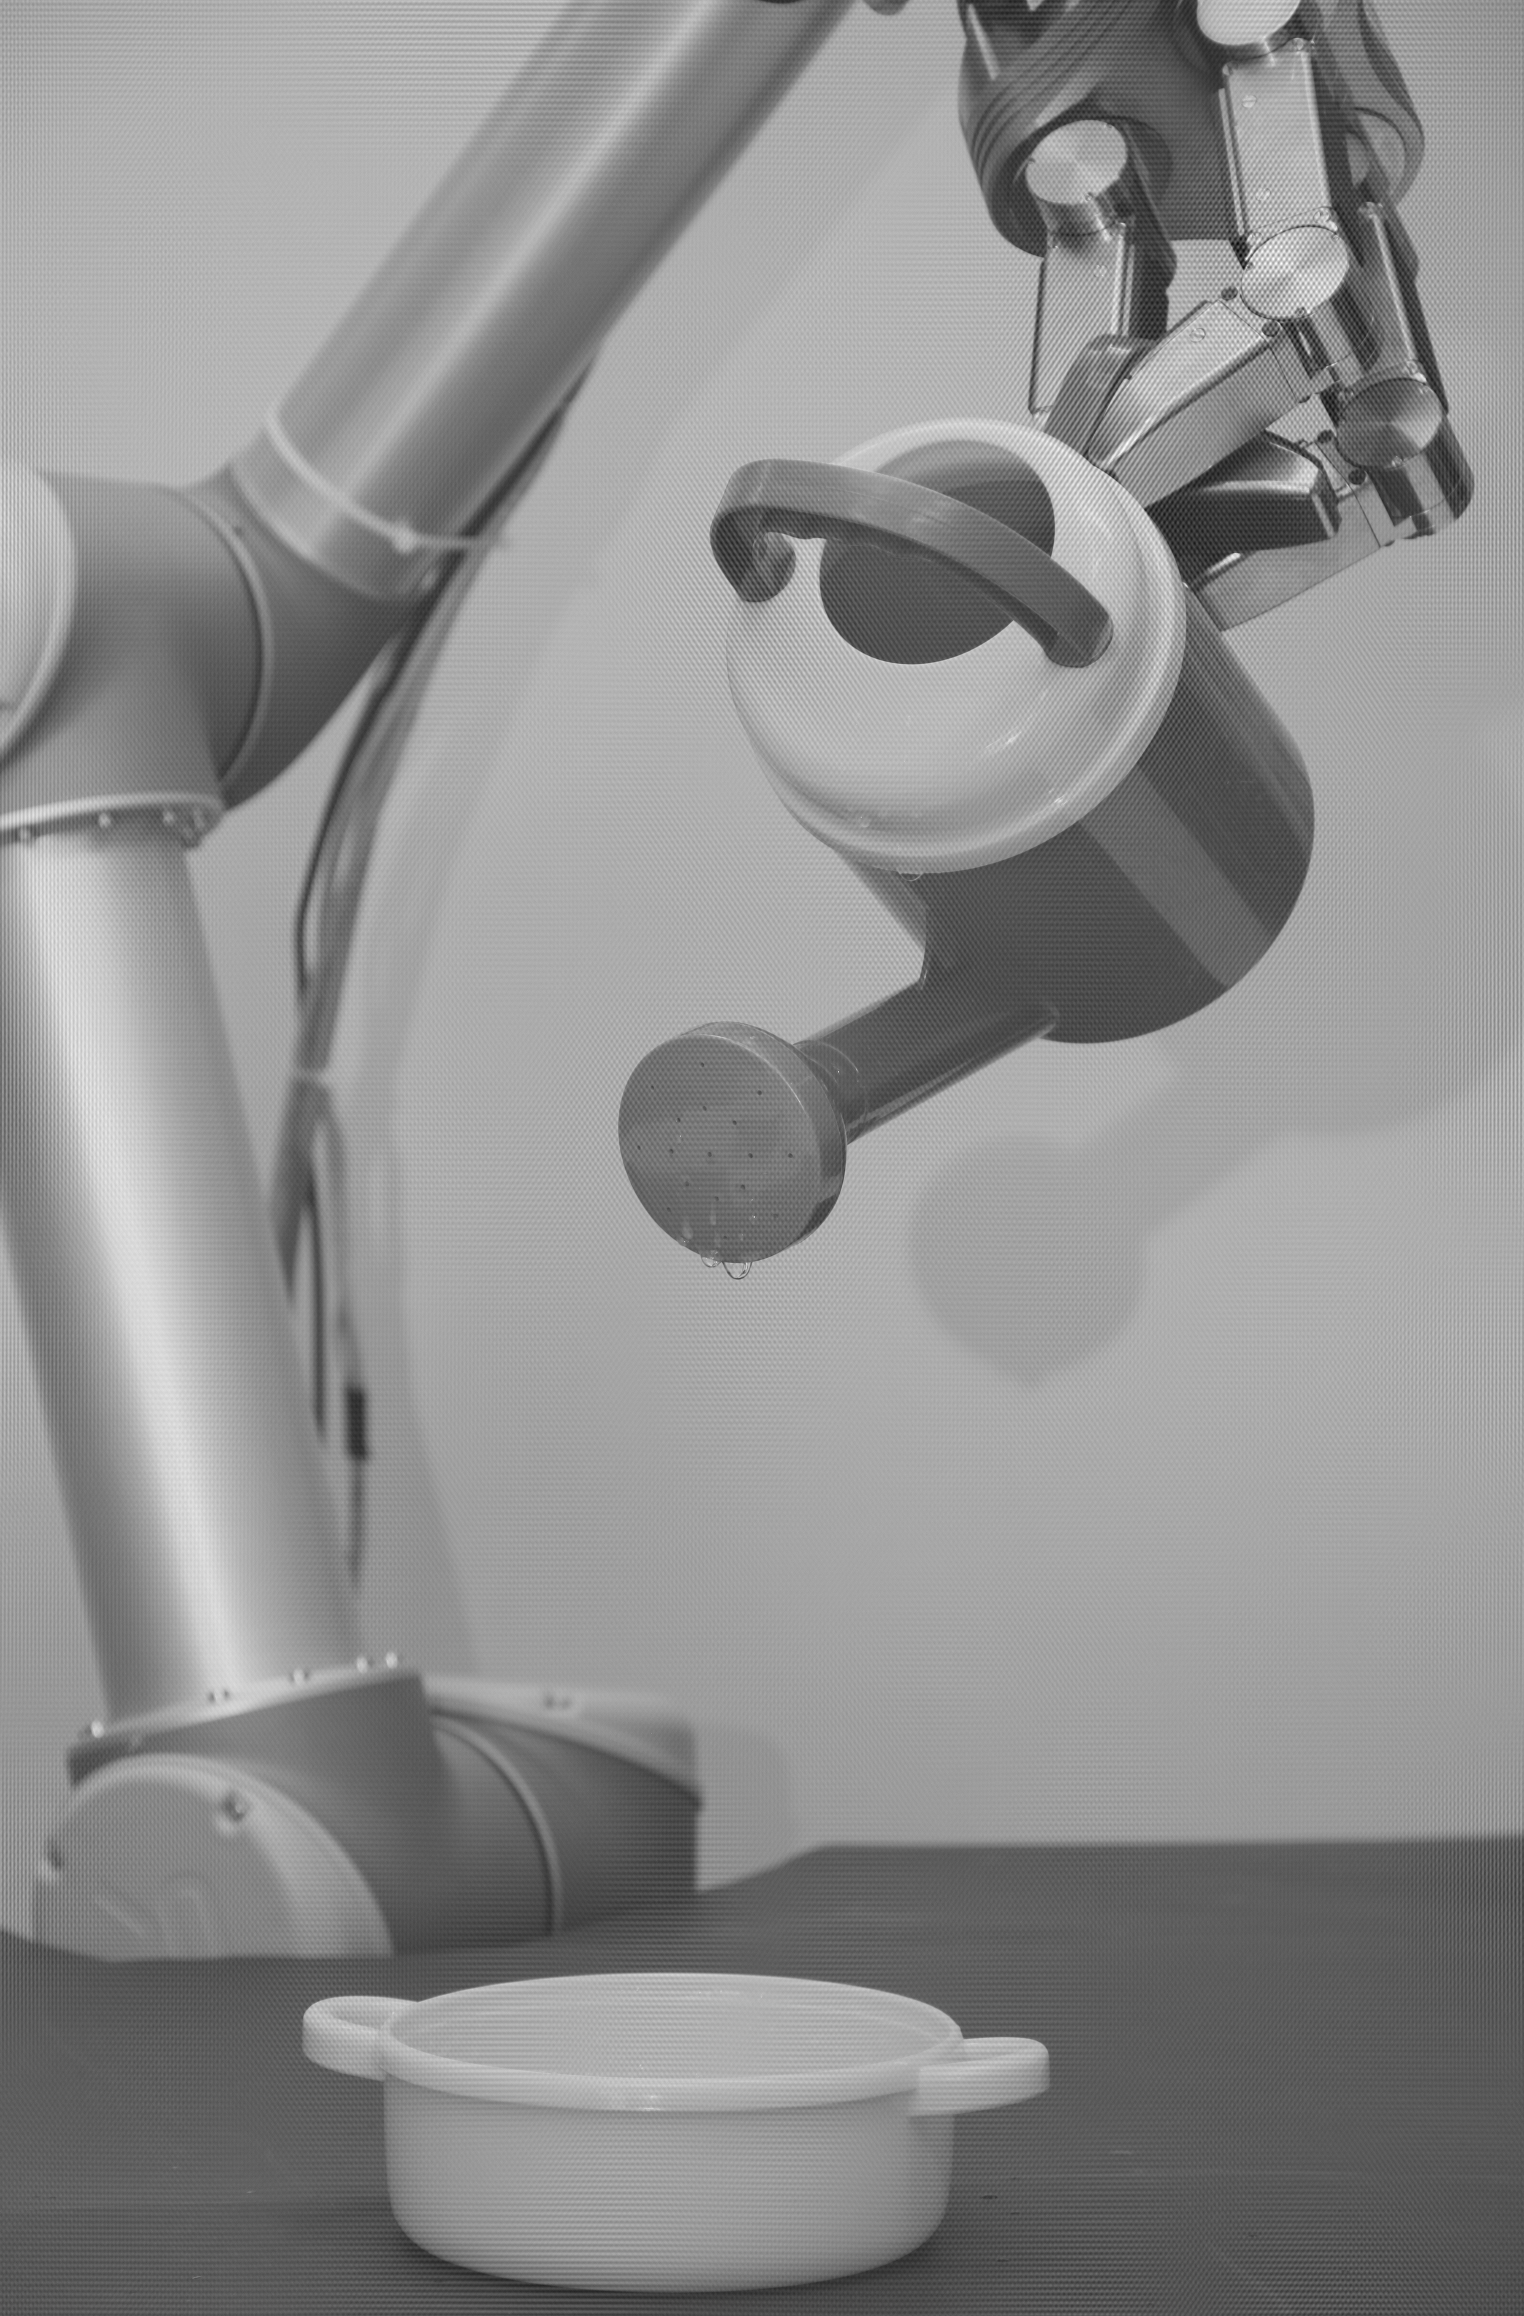
\includegraphics[width=\textwidth]{img4/Image4_2.png}
        \caption{Image4\_2 with \\no restoration}
        \label{fig:img42_src}
    \end{subfigure}
    \begin{subfigure}[b]{0.23\textwidth}
        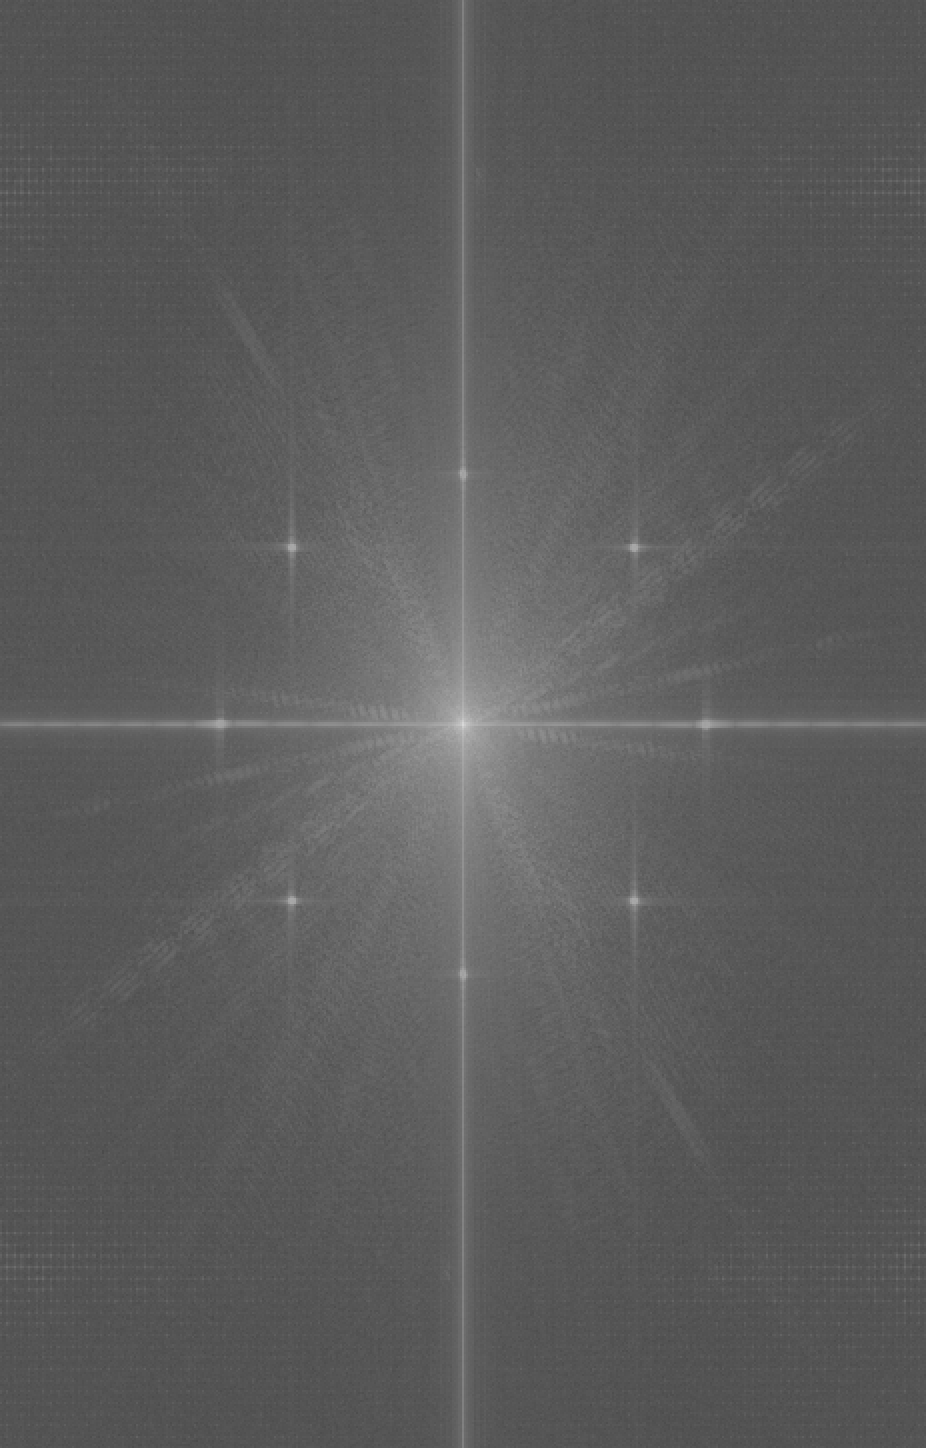
\includegraphics[width=\textwidth]{img4/Image4_2_freq_spec.png}
        \caption{Frequency spectrum of Image4\_2}
        \label{fig:img1_hist}
    \end{subfigure}
    \caption{Analysis of image 1}\label{fig:img1}
\end{figure}

The frequency components creating the circle are reason why the the stripes are occuring in the image.  One way of resolving this issue is to create a low pass filter, which let everything below a certain frequency pass, and the filter frequencies above away. \\

One type of lowpass filter is the butterworth lowpass filter which is defined as
\begin{equation}
	H(u,v) = \frac{1}{1+[\frac{D(u,v)}{D_0}]^{2n}}
	\label{eq:LBP}
	\cite{Bogen side 295}
\end{equation}
\todo{Cite til bogen side 295}
$D_0$ is the cutoff frequency given as the distance from the origin, n  is the order,  and D(u,v) is distance between a point (u,v) in the frequency domain and the center frequency rectangle, it is calculated as such. 

\begin{equation}
D(u,v) = [(u-P/2)^2 + (v-Q/2)^2]^{\frac{1}{2}} 
\end{equation}

P and Q is the padded size of the rectangle. \\


The cutoff frequency can easily by found, by computing the distance between the origin and the corresponding frequency component. The origin i as the pixel position $(1536 ,2408)$, and one of the undesired frequency component lies as pixel position $(2336,2400)$ \\


This distance is computed to be 800, which means that $D_0$ below 800, should be able to filter out the frequency components causing the stripes. \\

\begin{figure}[H]
    \centering
    \begin{subfigure}[b]{0.16\textwidth}
        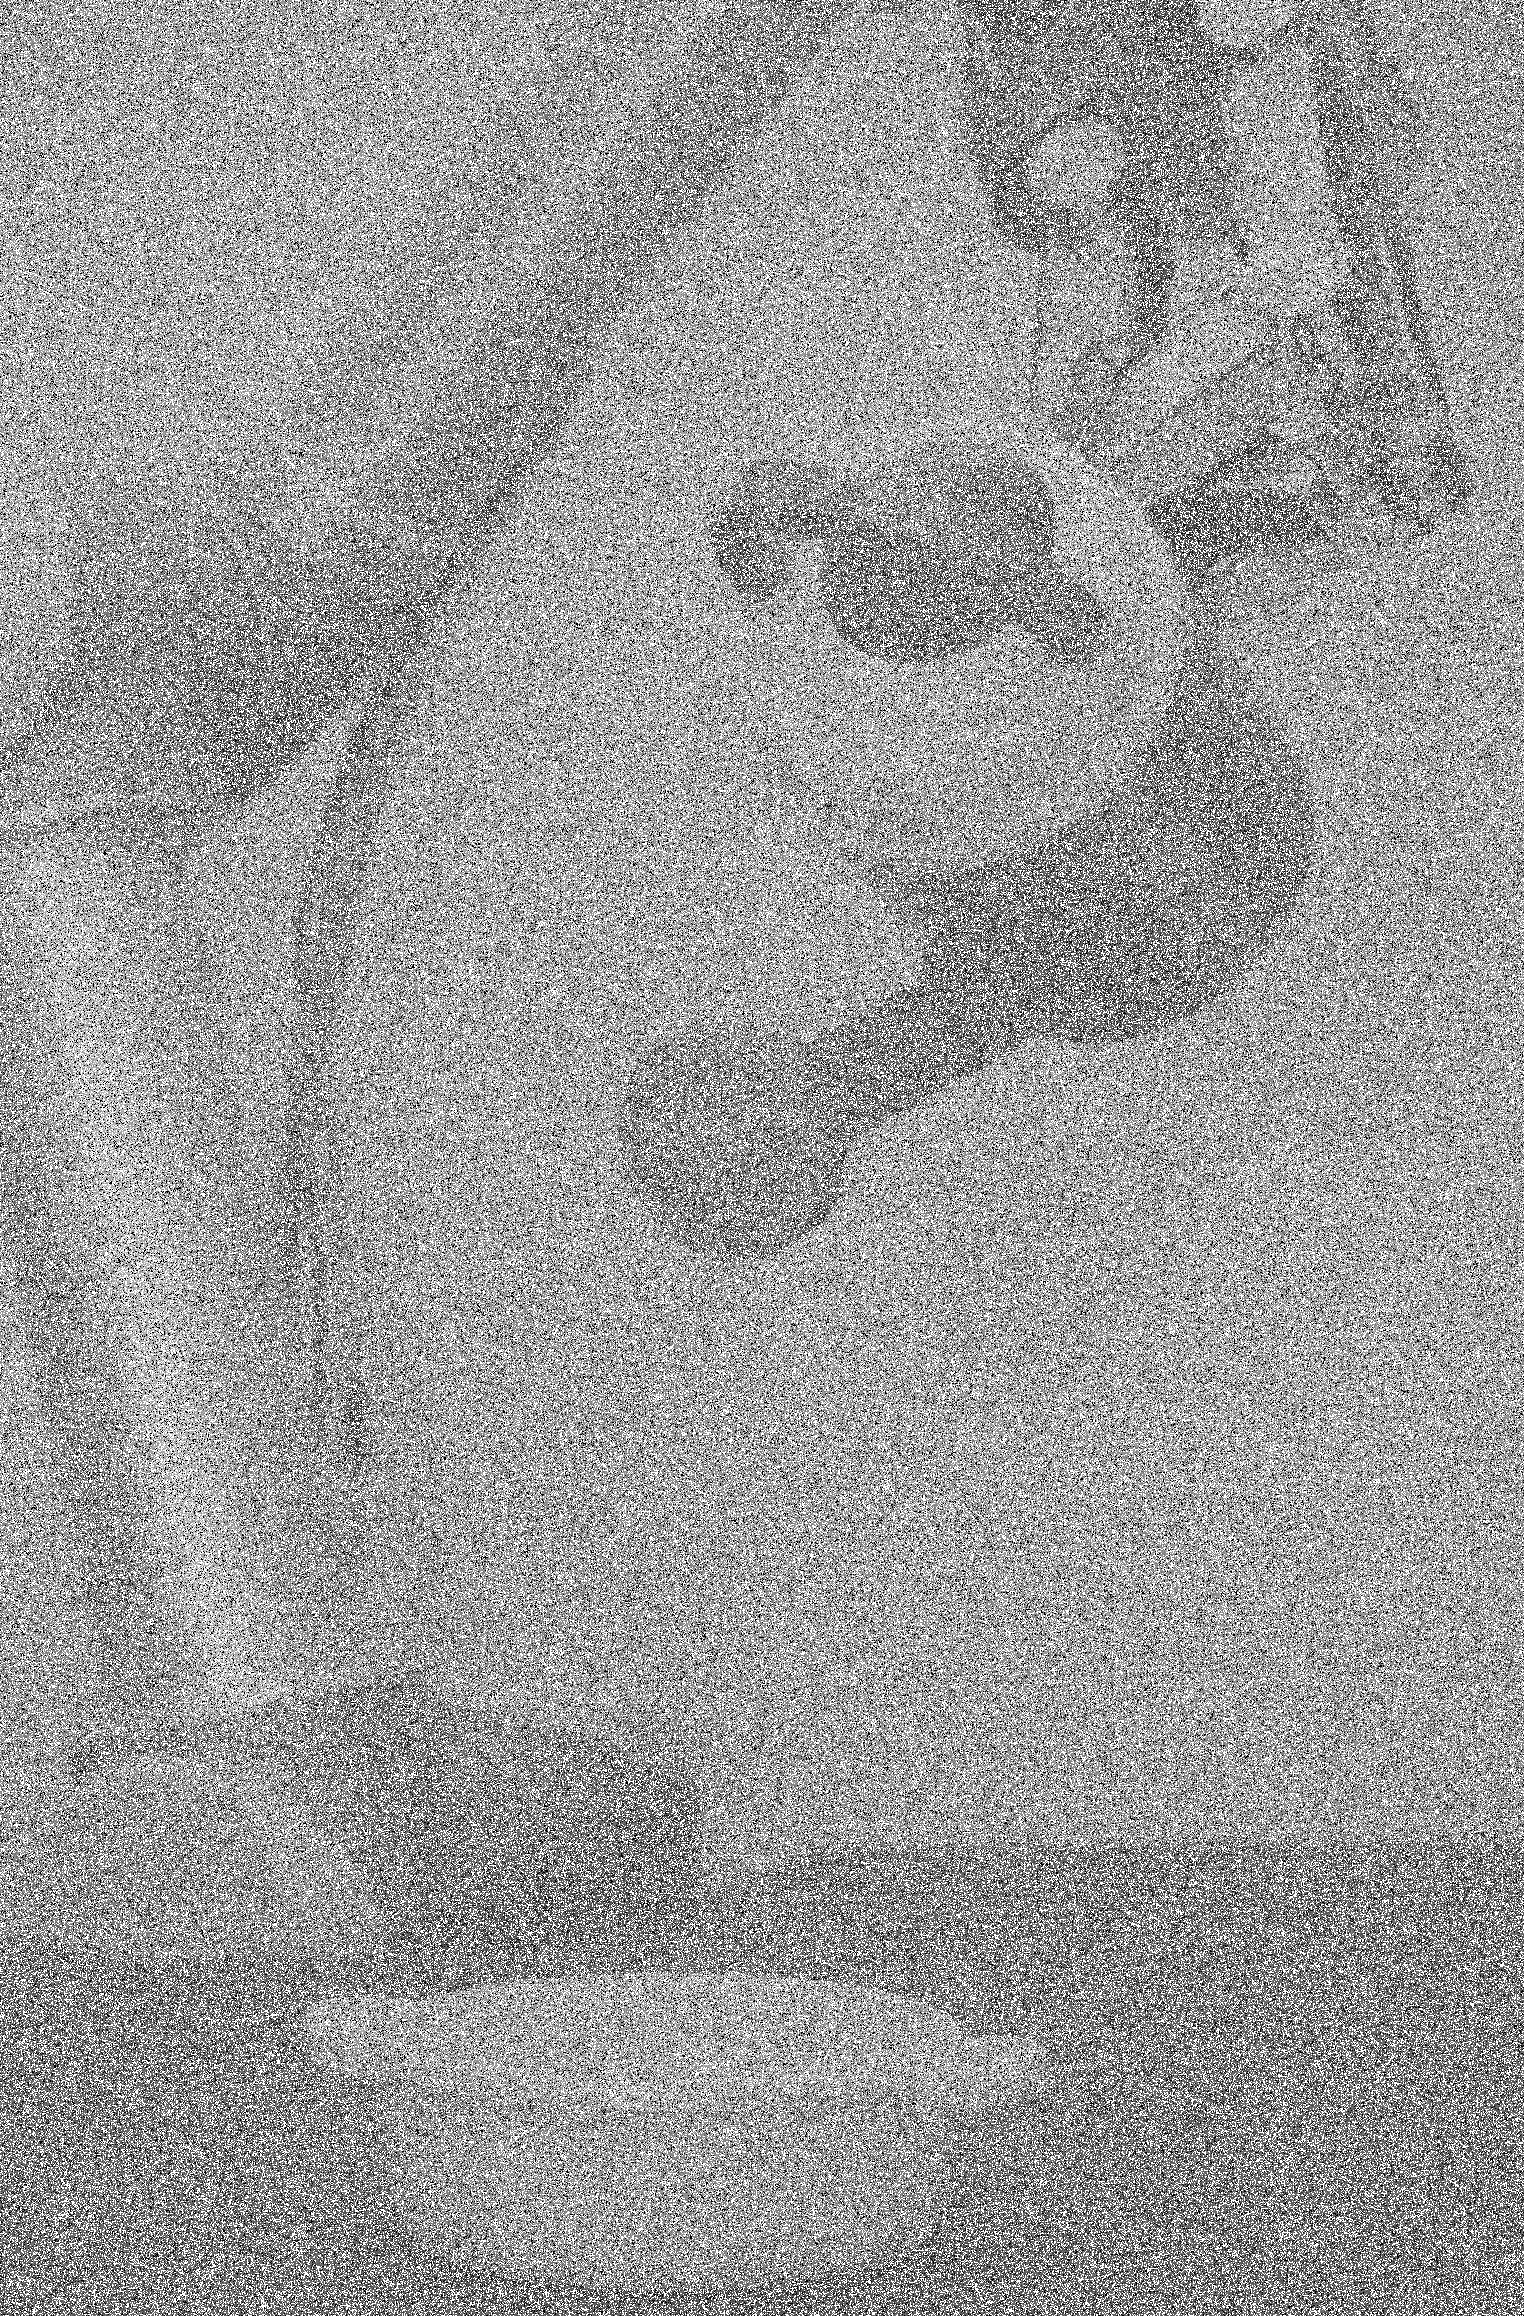
\includegraphics[width=\textwidth]{img2/src.png}
        \caption{The original image}
        \label{fig:img2_src}
    \end{subfigure}
    \begin{subfigure}[b]{0.16\textwidth}
        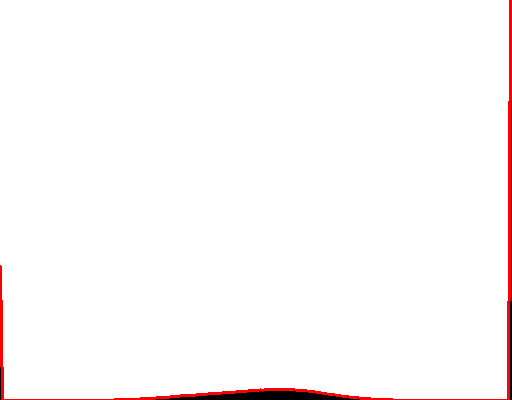
\includegraphics[width=\textwidth]{img2/hist.png}
        \caption{Histogram of the original image}
        \label{fig:img2_hist}
    \end{subfigure}
	 \begin{subfigure}[b]{0.16\textwidth}
        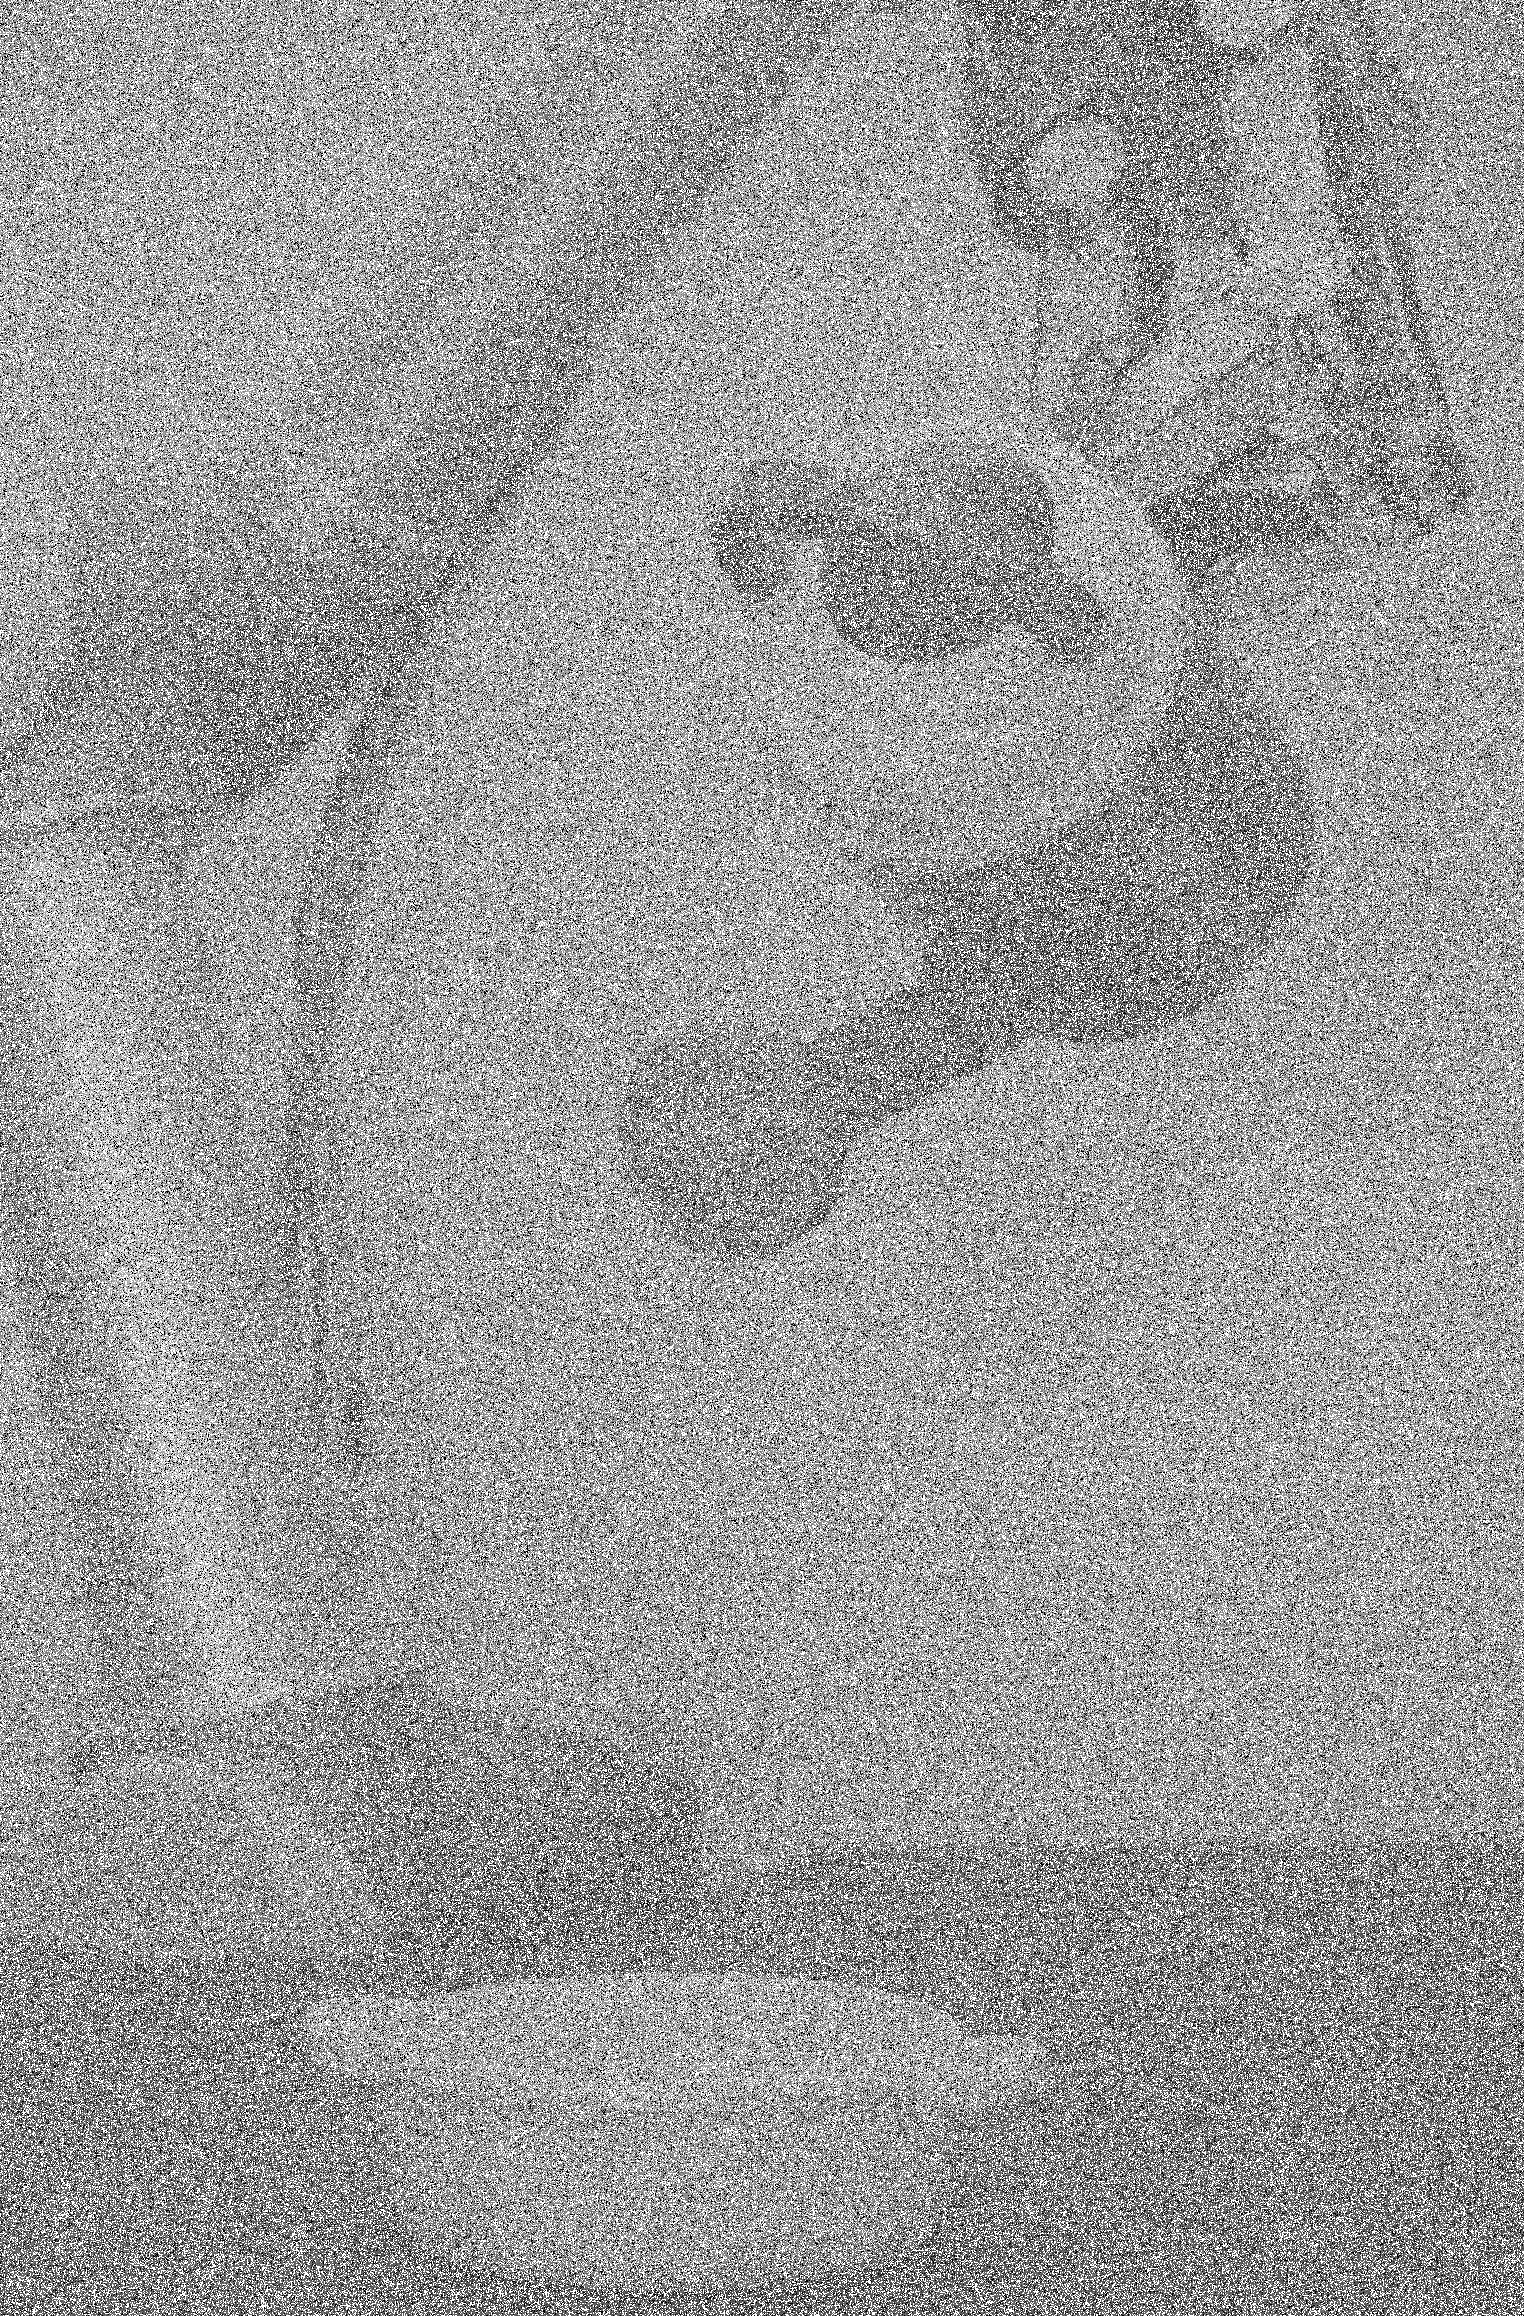
\includegraphics[width=\textwidth]{img2/src.png}
        \caption{The original image}
        \label{fig:img2_src}
    \end{subfigure}
    \begin{subfigure}[b]{0.16\textwidth}
        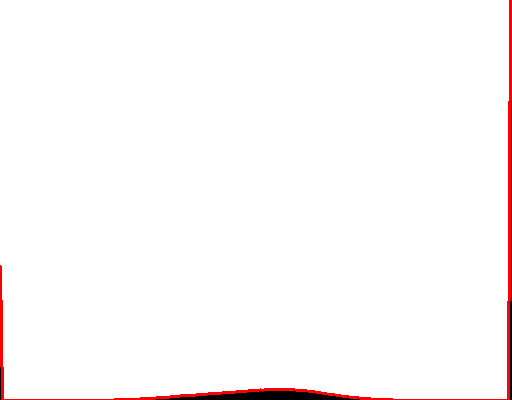
\includegraphics[width=\textwidth]{img2/hist.png}
        \caption{Histogram of the original image}
        \label{fig:img2_hist}
    \end{subfigure}	
\begin{subfigure}[b]{0.16\textwidth}
        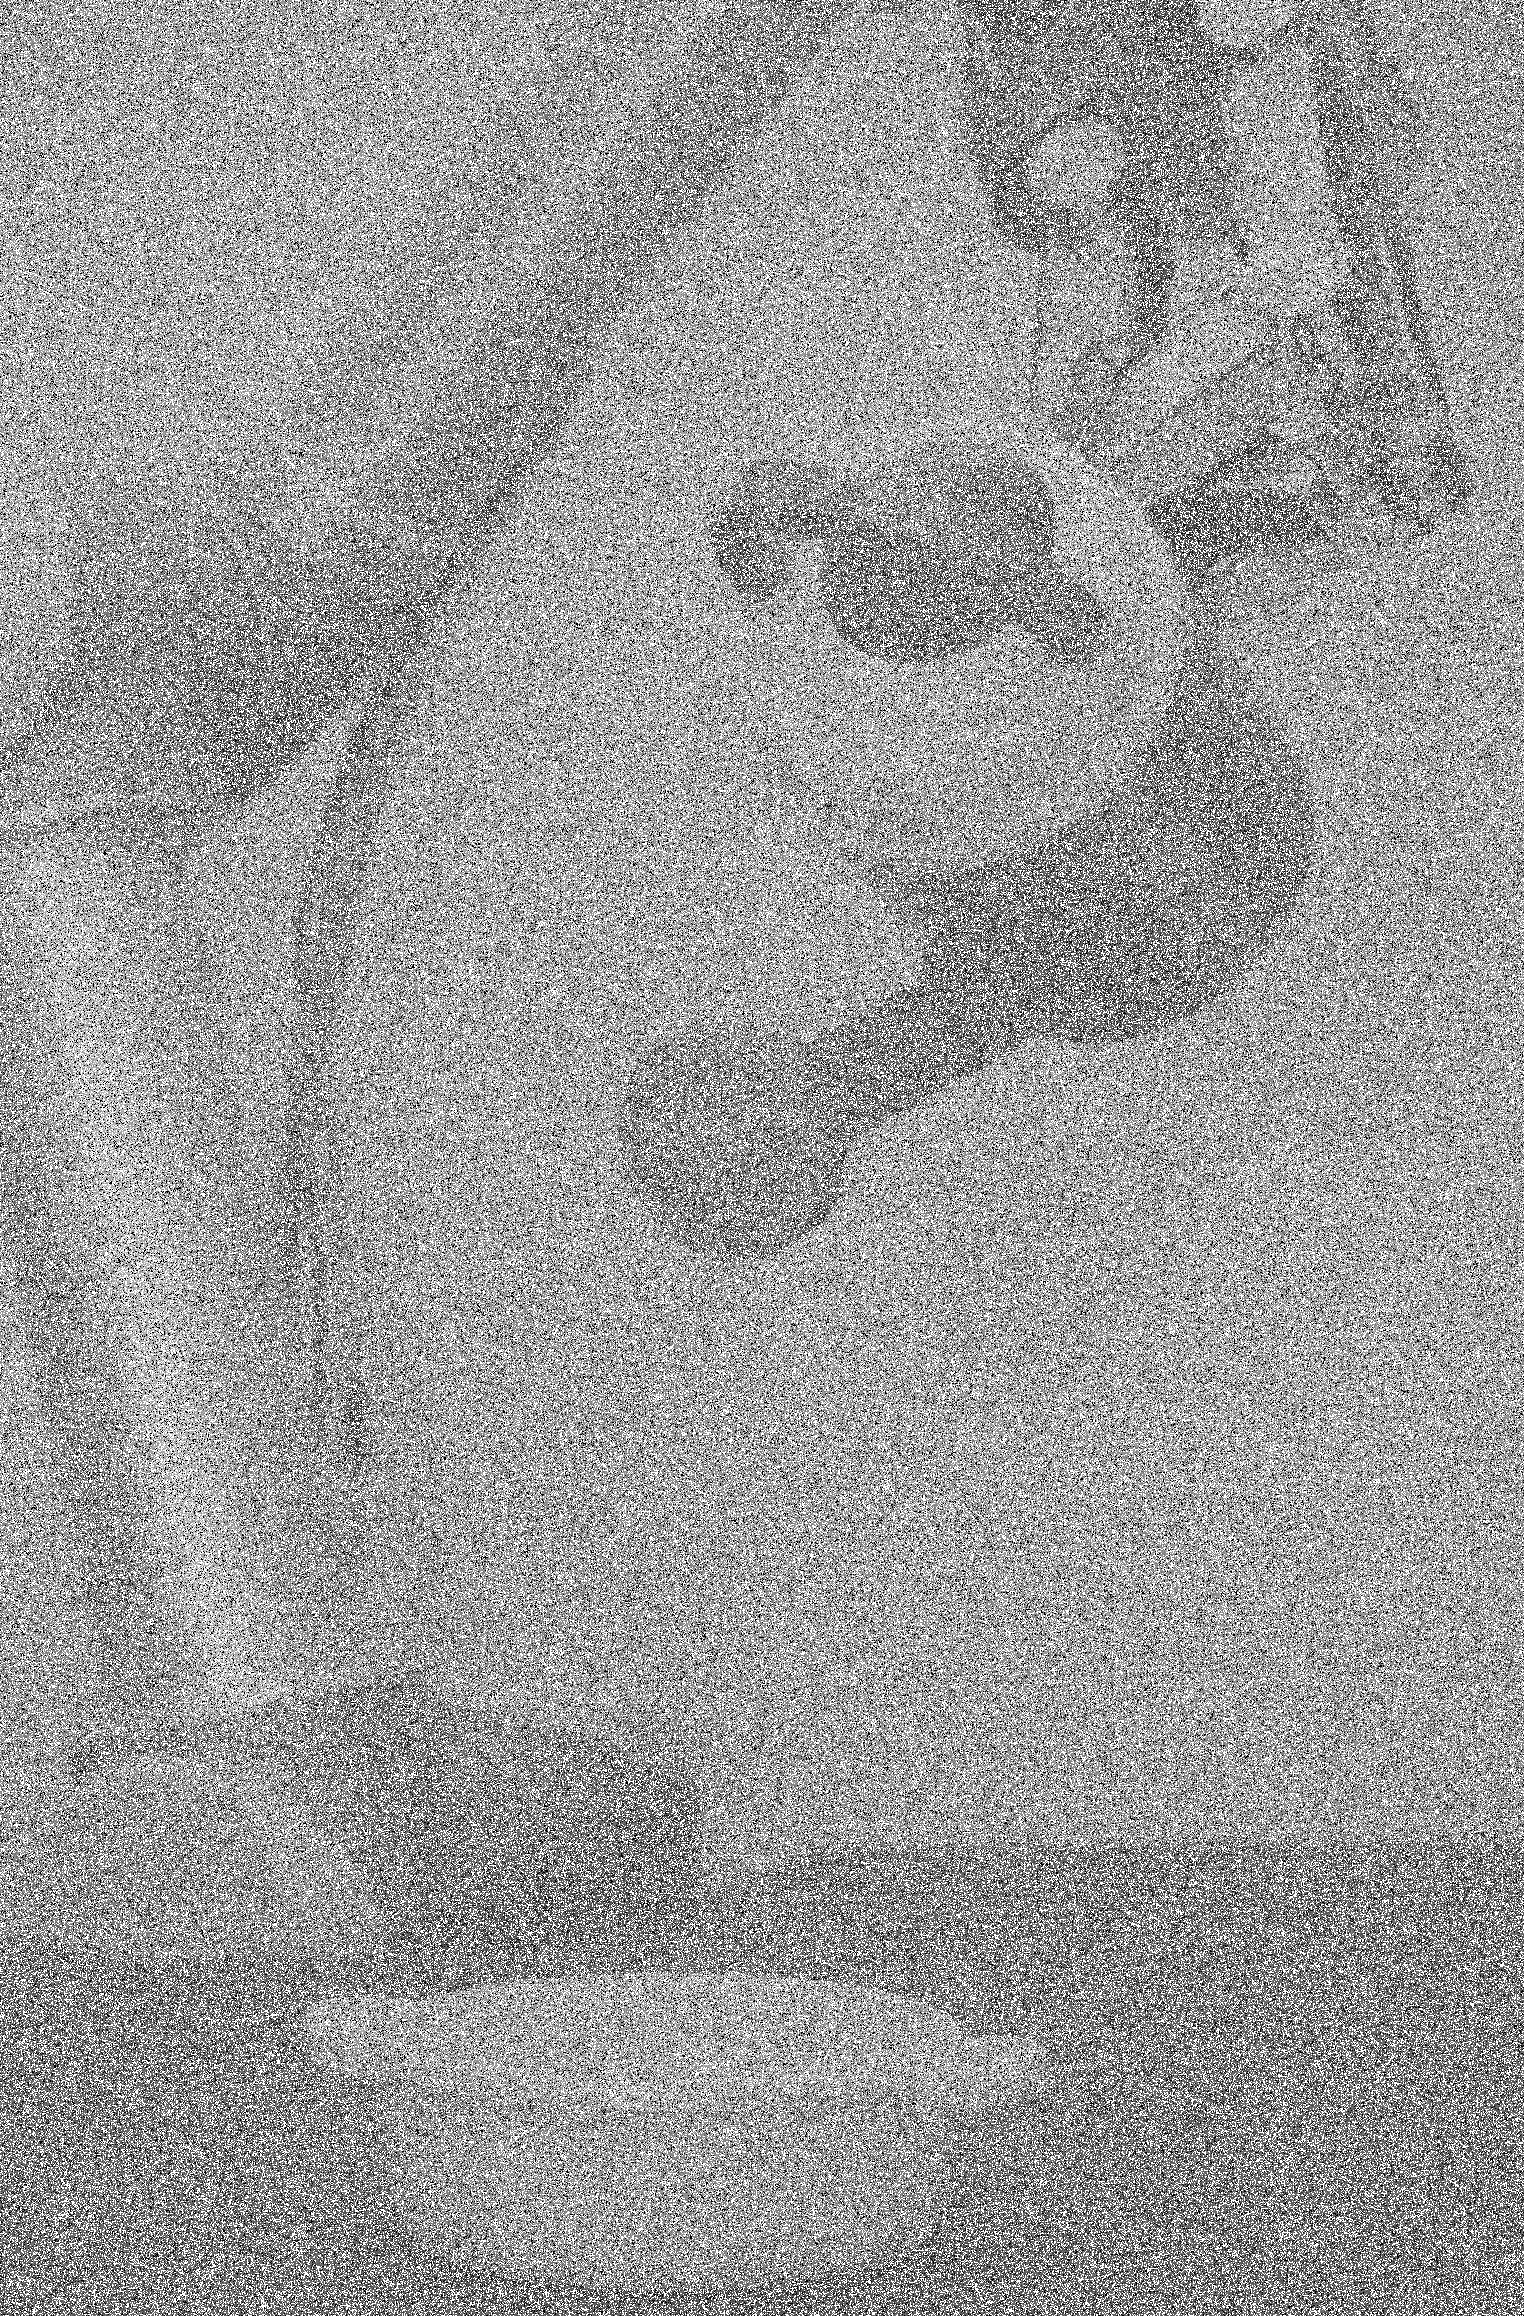
\includegraphics[width=\textwidth]{img2/src.png}
        \caption{The original image}
        \label{fig:img2_src}
    \end{subfigure}
    \begin{subfigure}[b]{0.16\textwidth}
        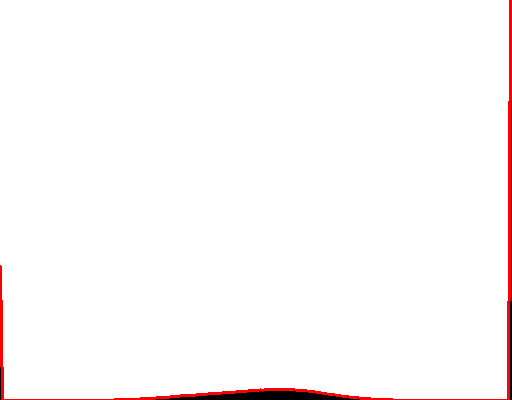
\includegraphics[width=\textwidth]{img2/hist.png}
        \caption{Histogram of the original image}
        \label{fig:img2_hist}
    \end{subfigure}	
    
    
      \begin{subfigure}[b]{0.16\textwidth}
        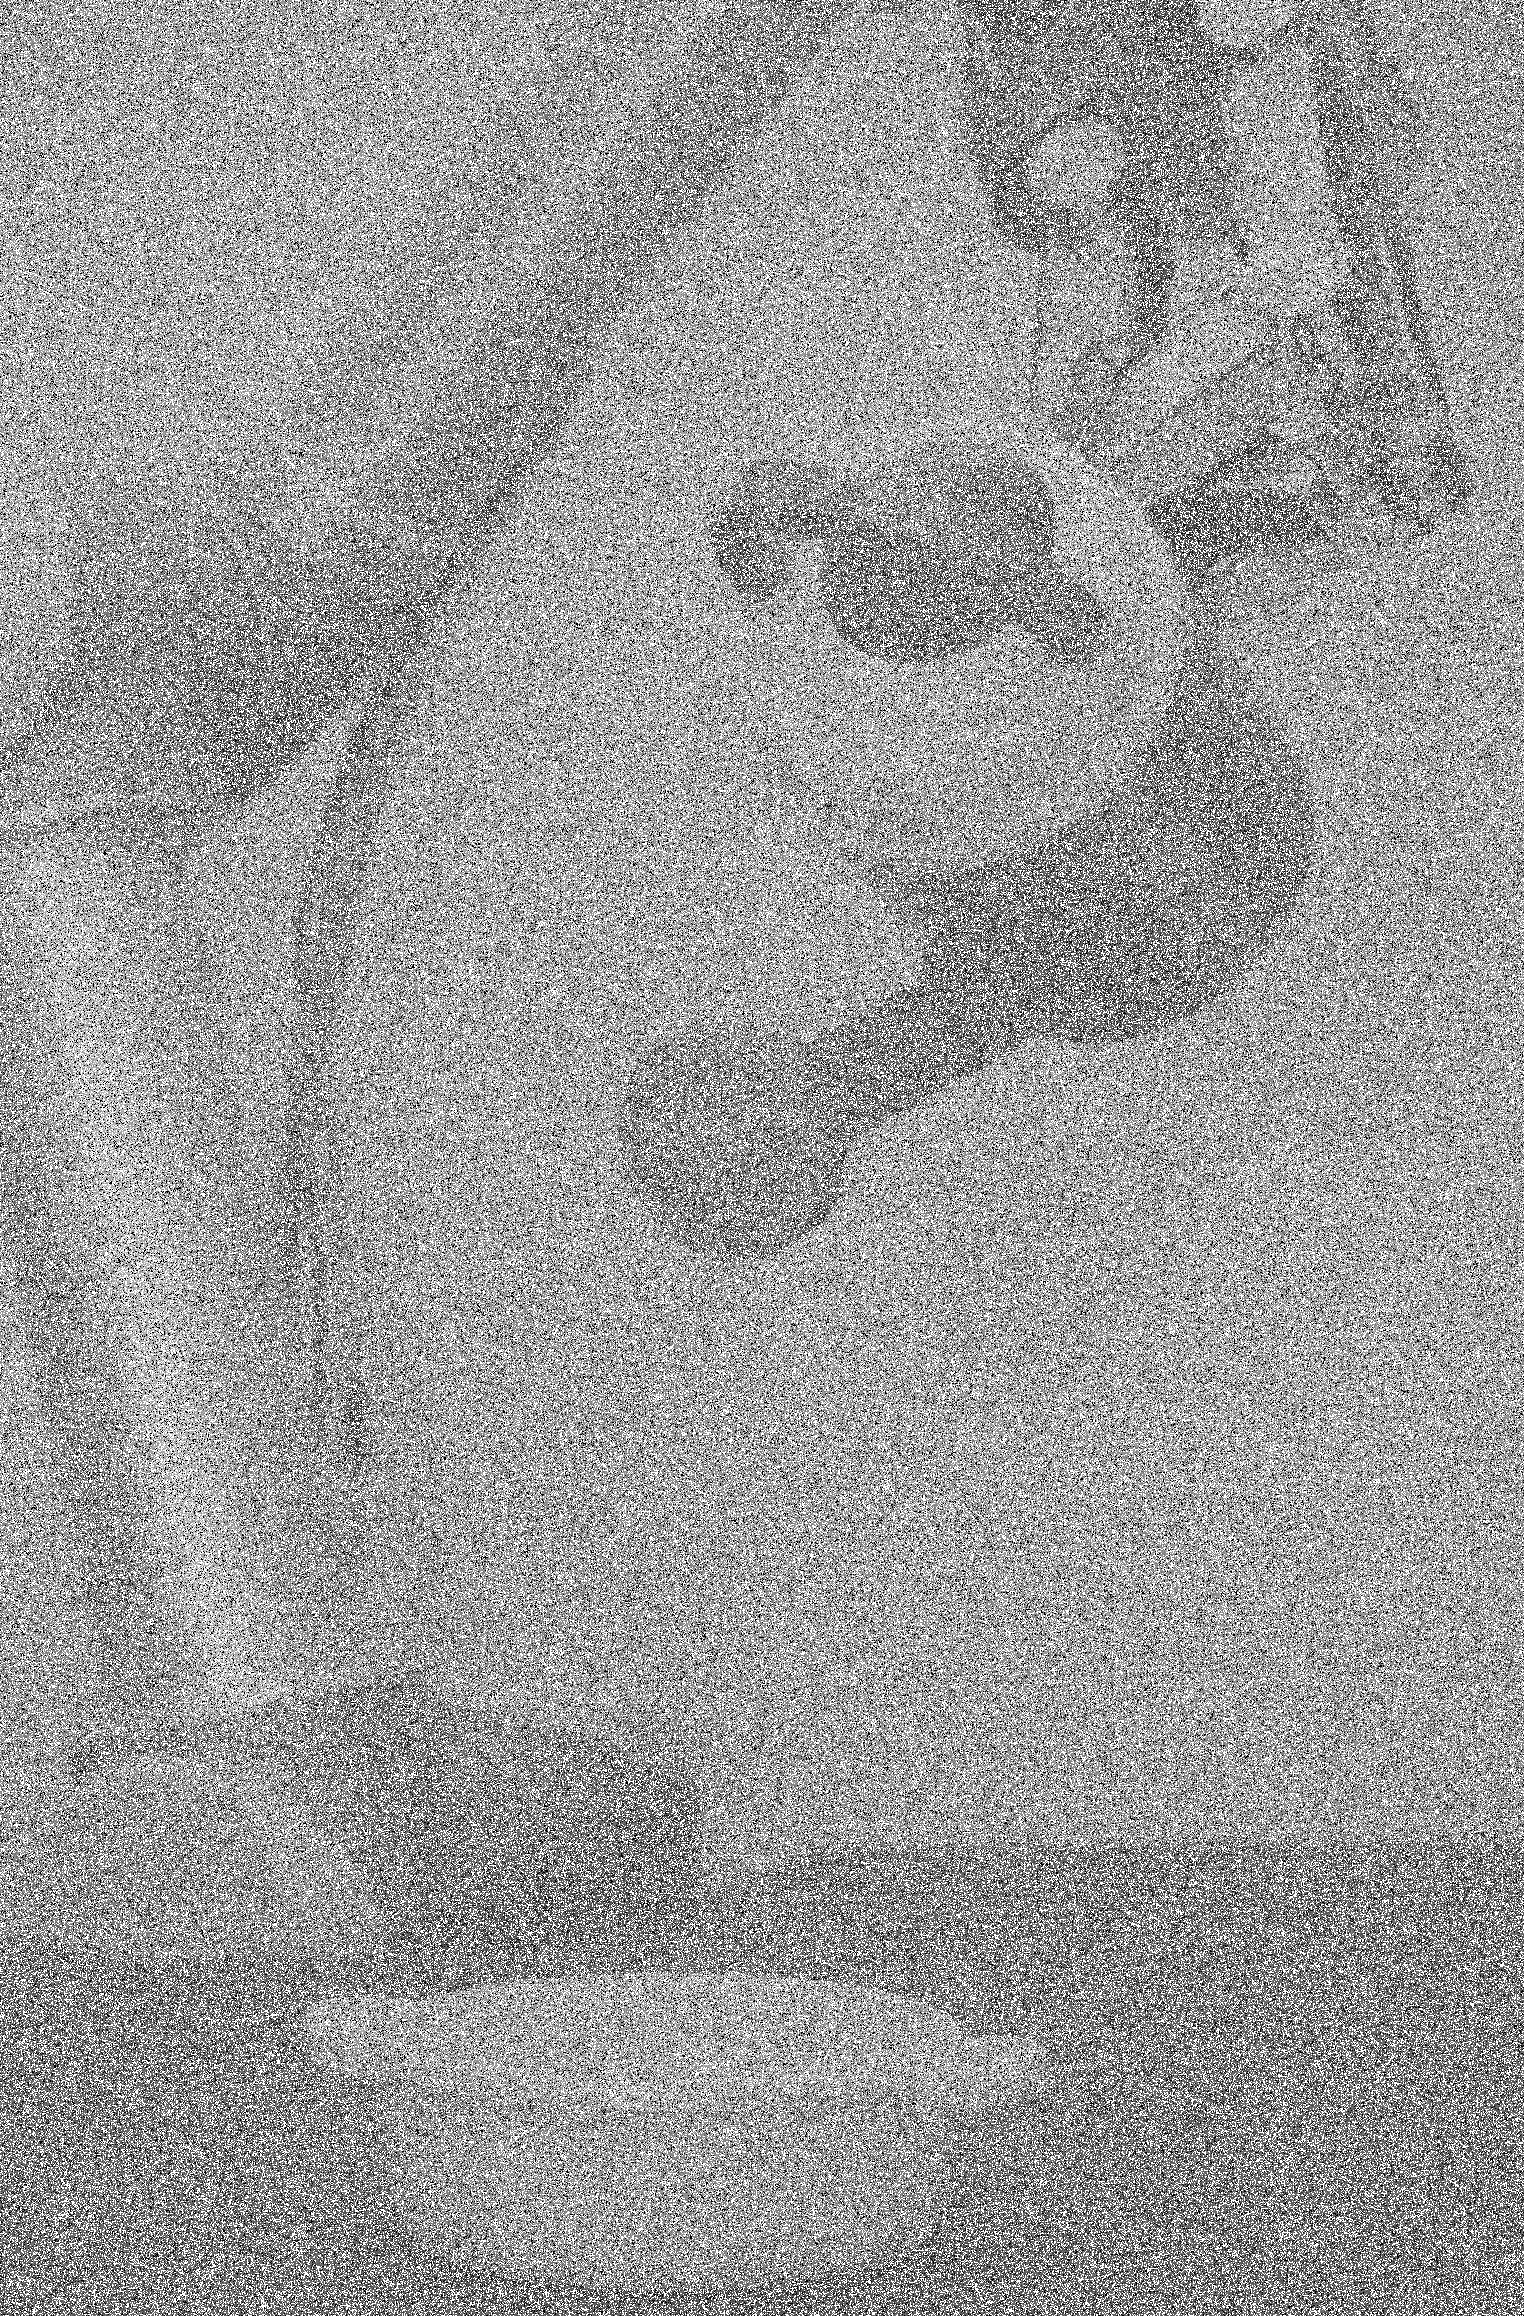
\includegraphics[width=\textwidth]{img2/src.png}
        \caption{The original image}
        \label{fig:img2_src}
    \end{subfigure}
    \begin{subfigure}[b]{0.16\textwidth}
        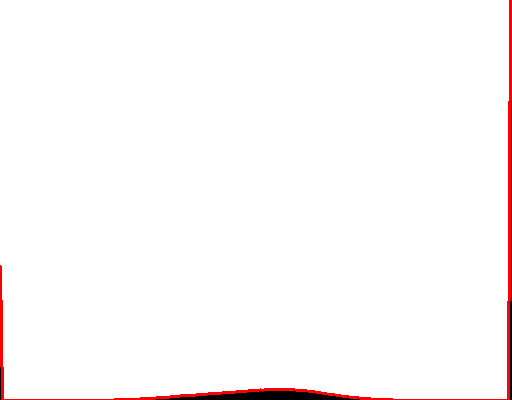
\includegraphics[width=\textwidth]{img2/hist.png}
        \caption{Histogram of the original image}
        \label{fig:img2_hist}
    \end{subfigure}
	 \begin{subfigure}[b]{0.16\textwidth}
        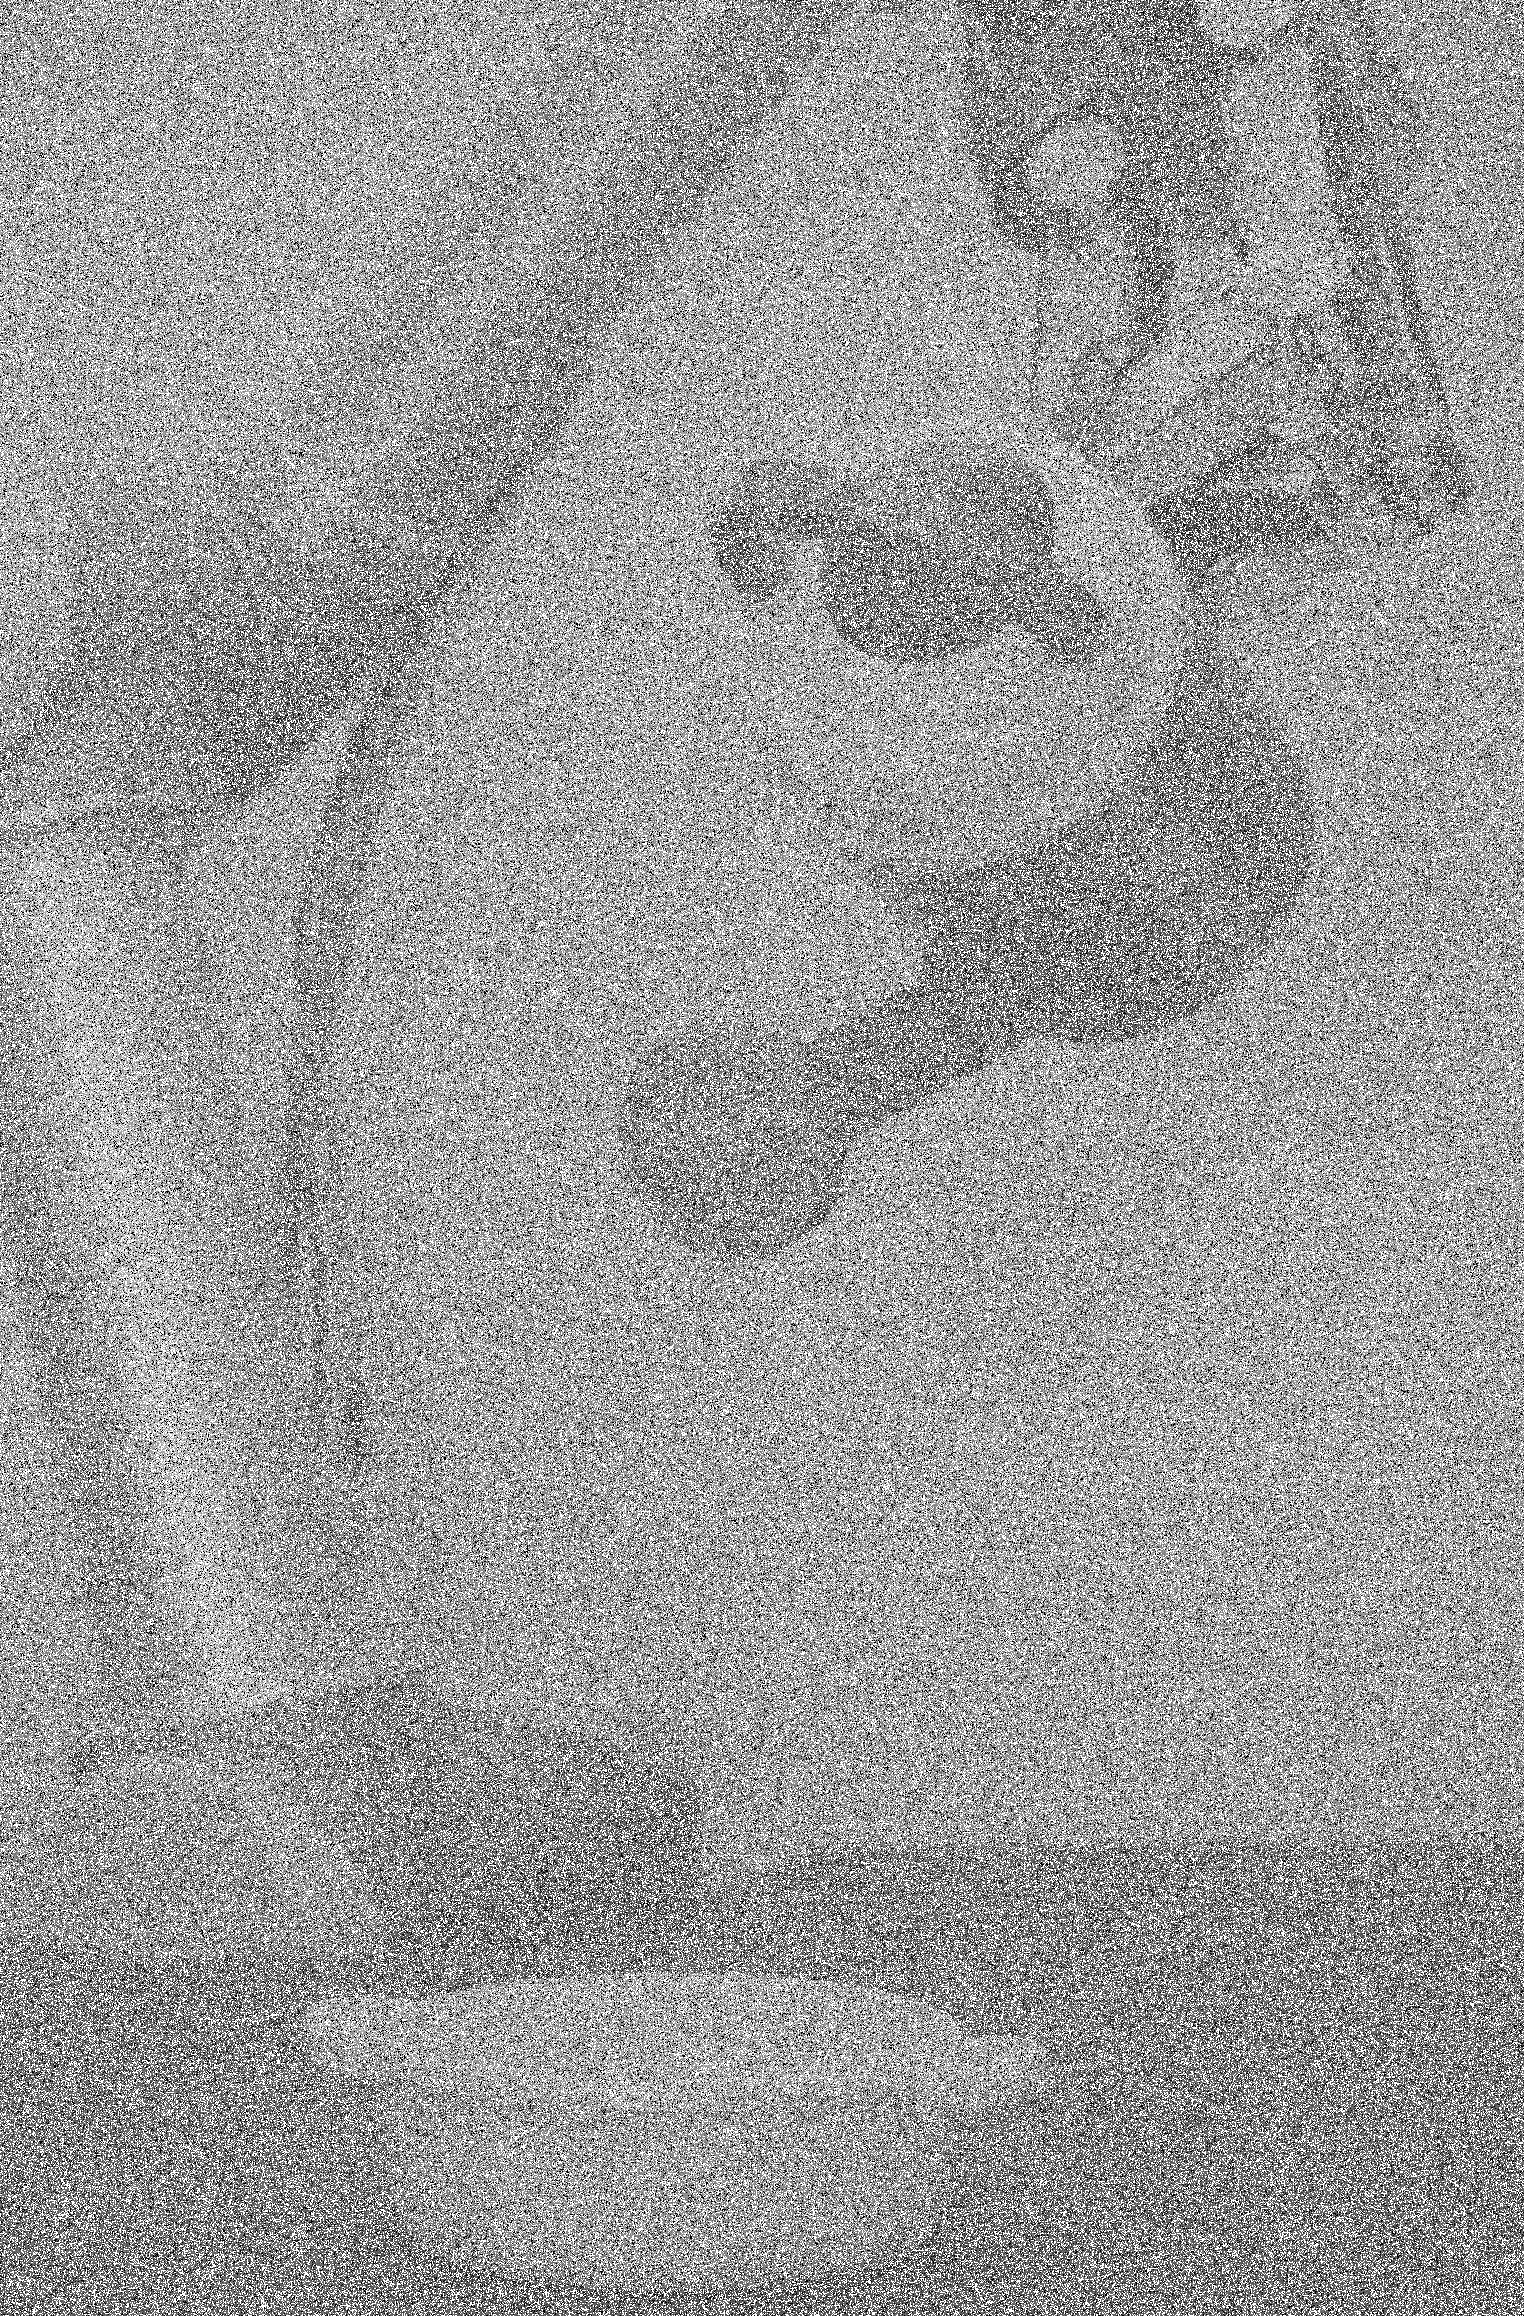
\includegraphics[width=\textwidth]{img2/src.png}
        \caption{The original image}
        \label{fig:img2_src}
    \end{subfigure}
    \begin{subfigure}[b]{0.16\textwidth}
        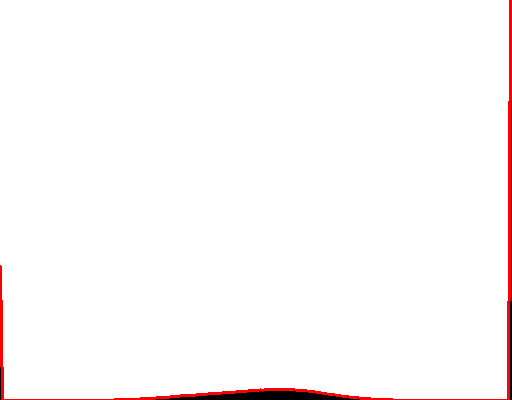
\includegraphics[width=\textwidth]{img2/hist.png}
        \caption{Histogram of the original image}
        \label{fig:img2_hist}
    \end{subfigure}	
\begin{subfigure}[b]{0.16\textwidth}
        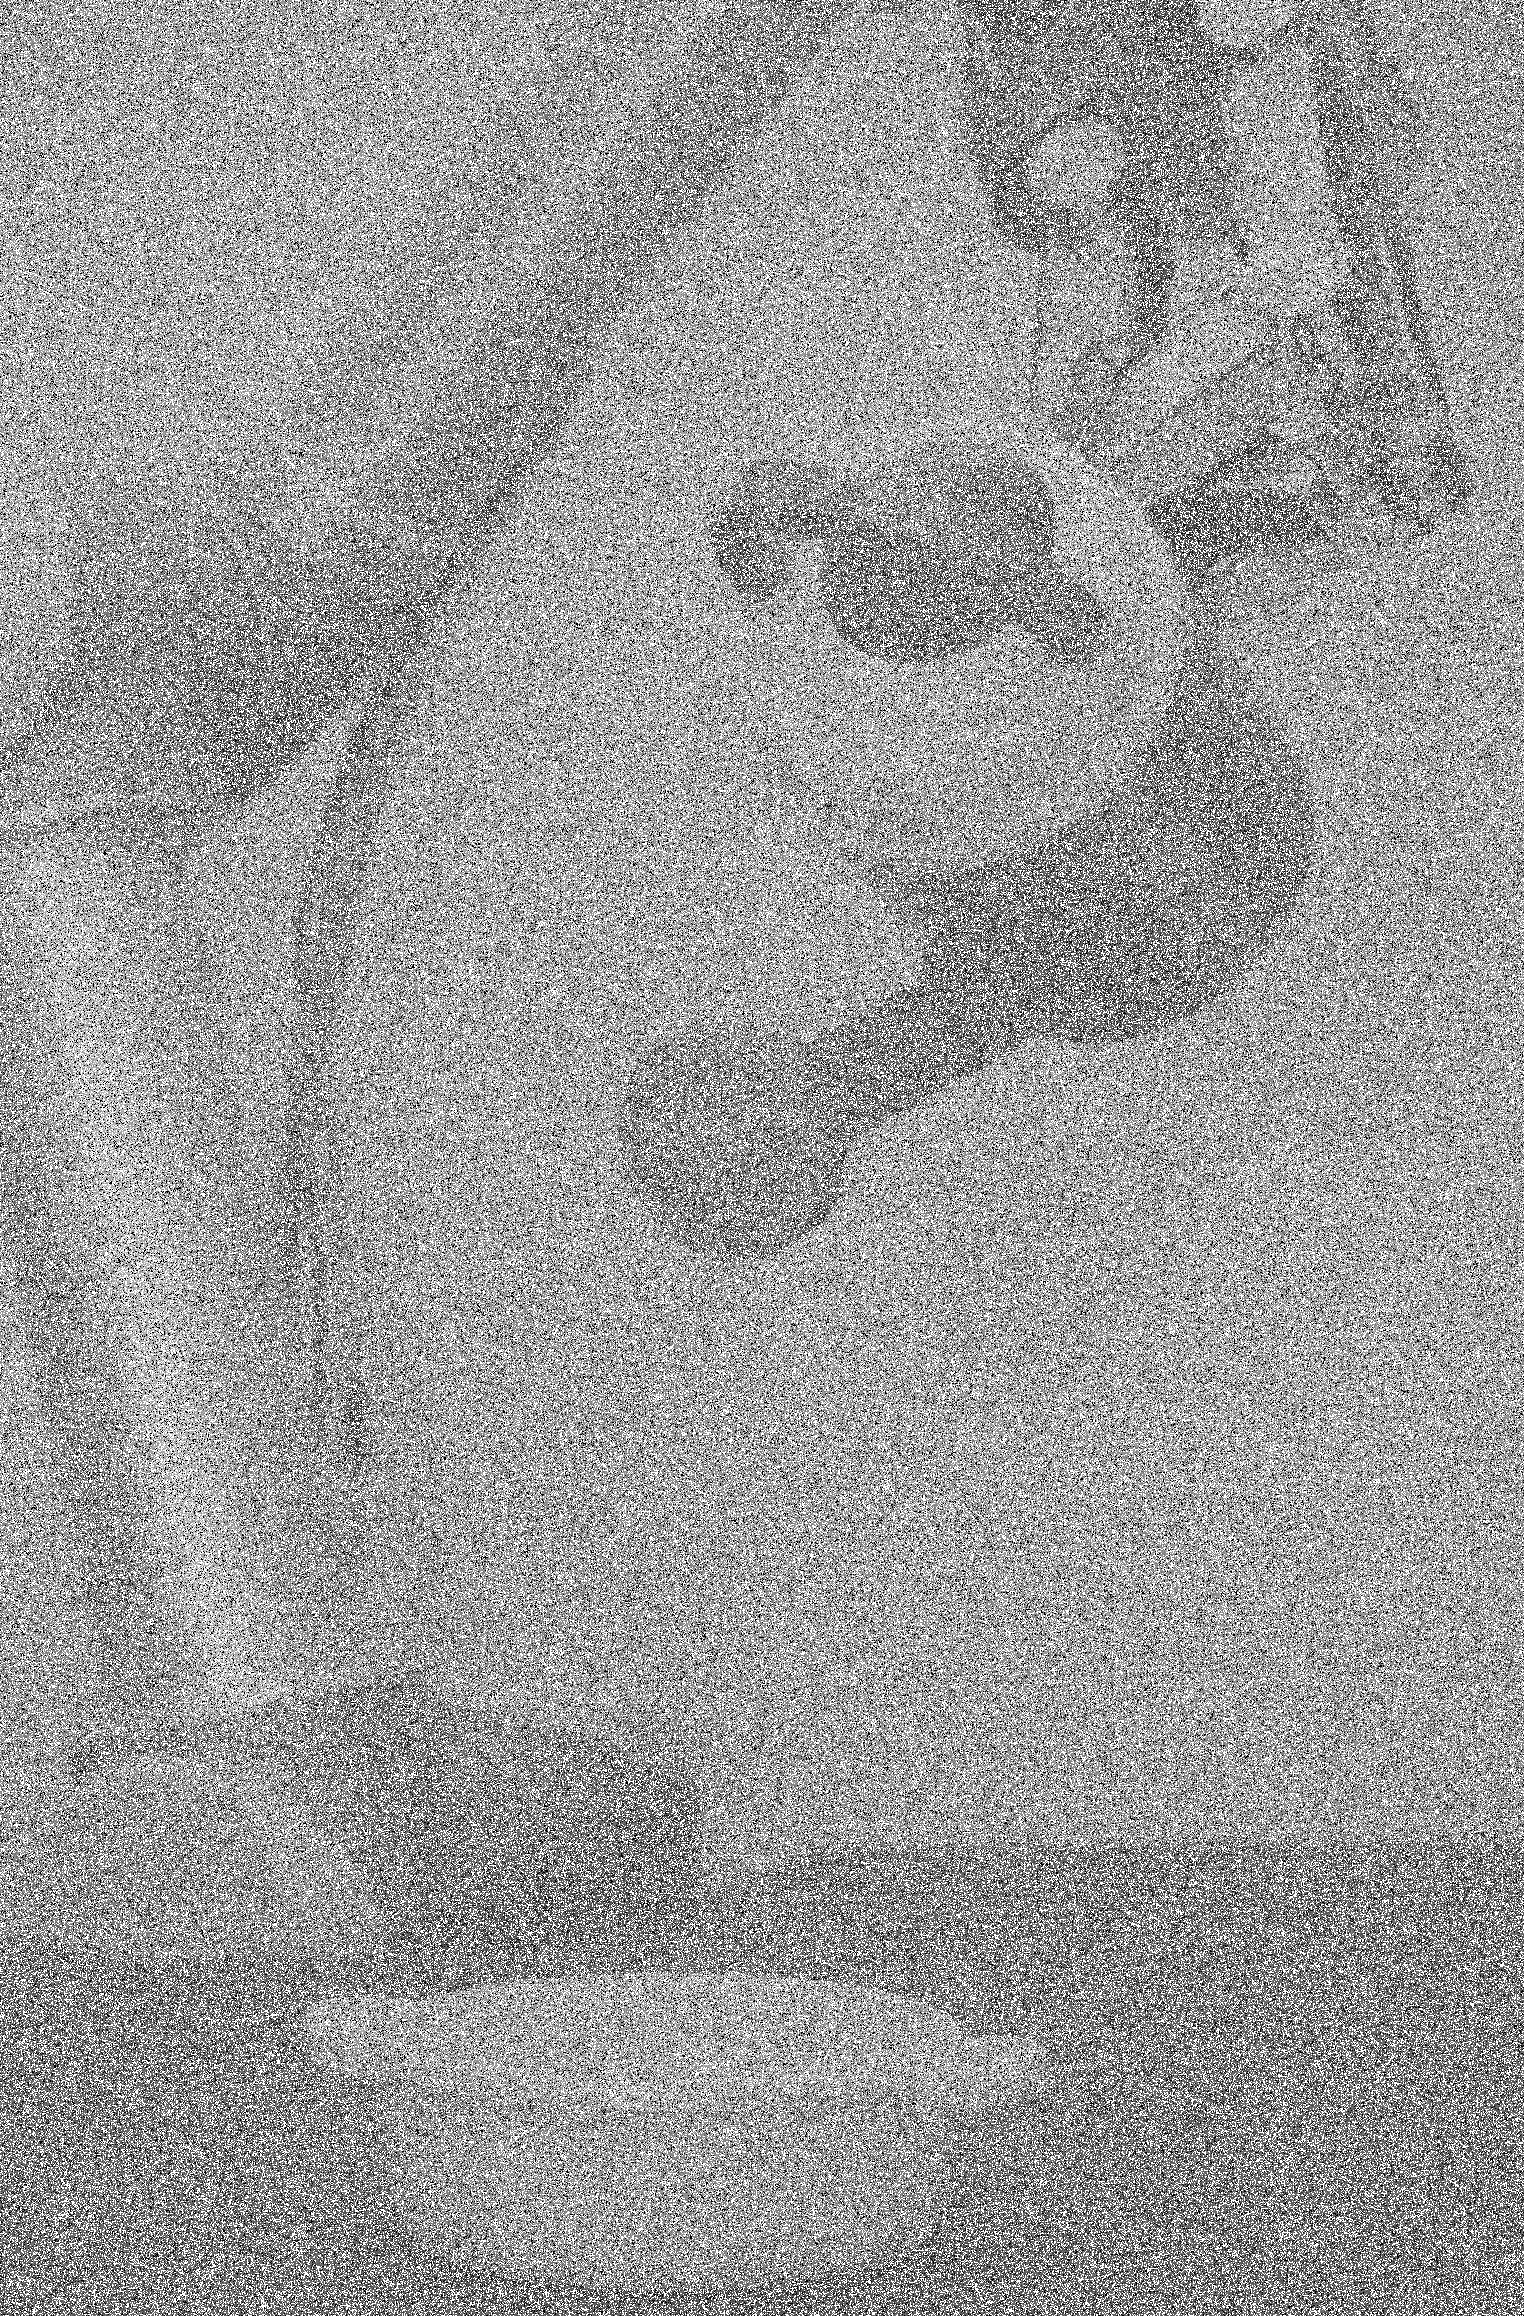
\includegraphics[width=\textwidth]{img2/src.png}
        \caption{The original image}
        \label{fig:img2_src}
    \end{subfigure}
    \begin{subfigure}[b]{0.16\textwidth}
        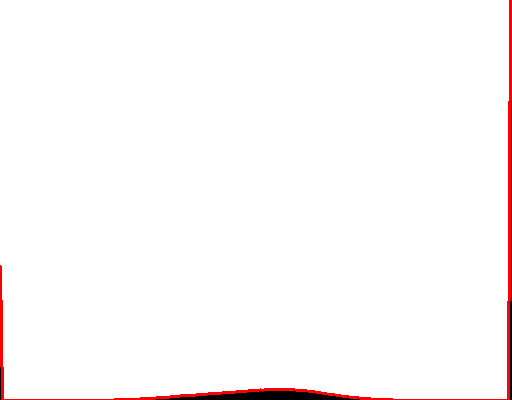
\includegraphics[width=\textwidth]{img2/hist.png}
        \caption{Histogram of the original image}
        \label{fig:img2_hist}
    \end{subfigure}
    
    
      \begin{subfigure}[b]{0.16\textwidth}
        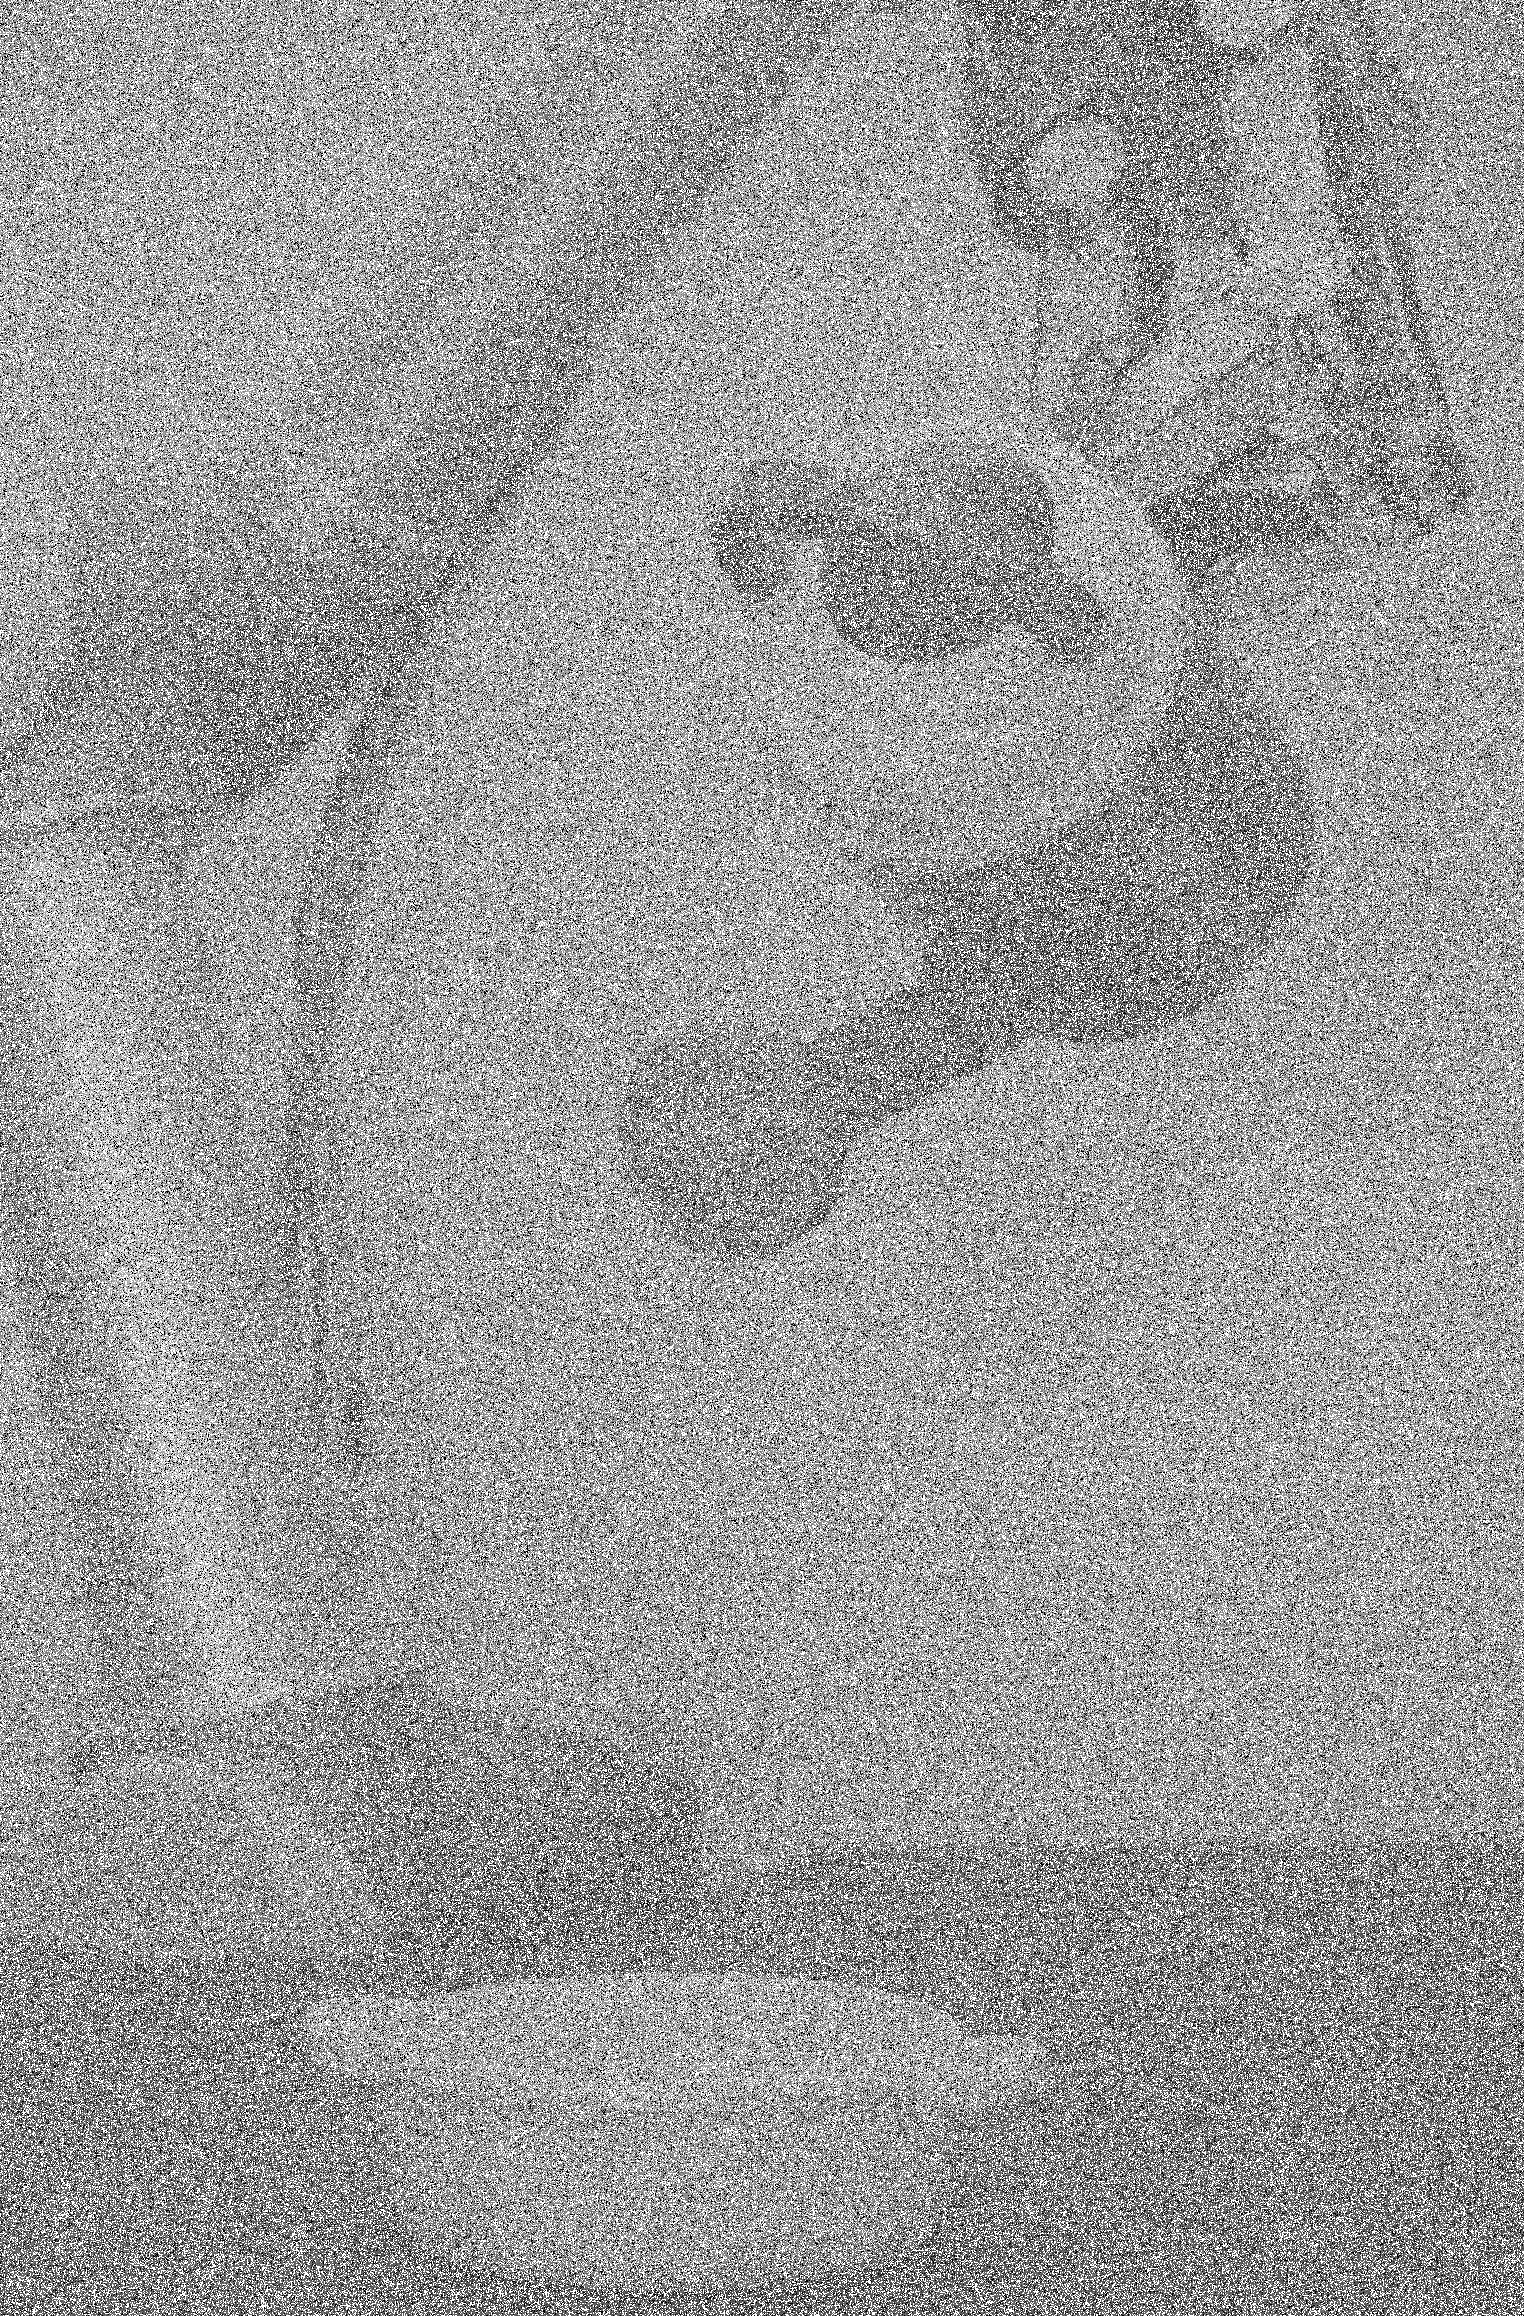
\includegraphics[width=\textwidth]{img2/src.png}
        \caption{The original image}
        \label{fig:img2_src}
    \end{subfigure}
    \begin{subfigure}[b]{0.16\textwidth}
        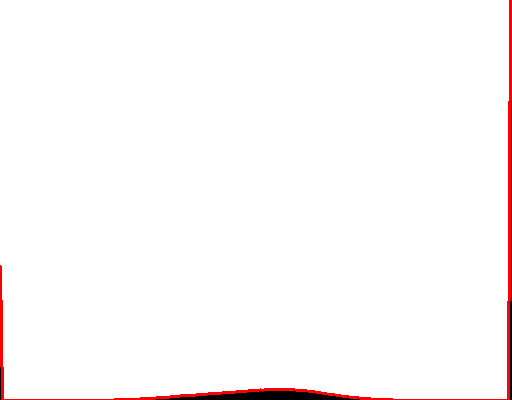
\includegraphics[width=\textwidth]{img2/hist.png}
        \caption{Histogram of the original image}
        \label{fig:img2_hist}
    \end{subfigure}
	 \begin{subfigure}[b]{0.16\textwidth}
        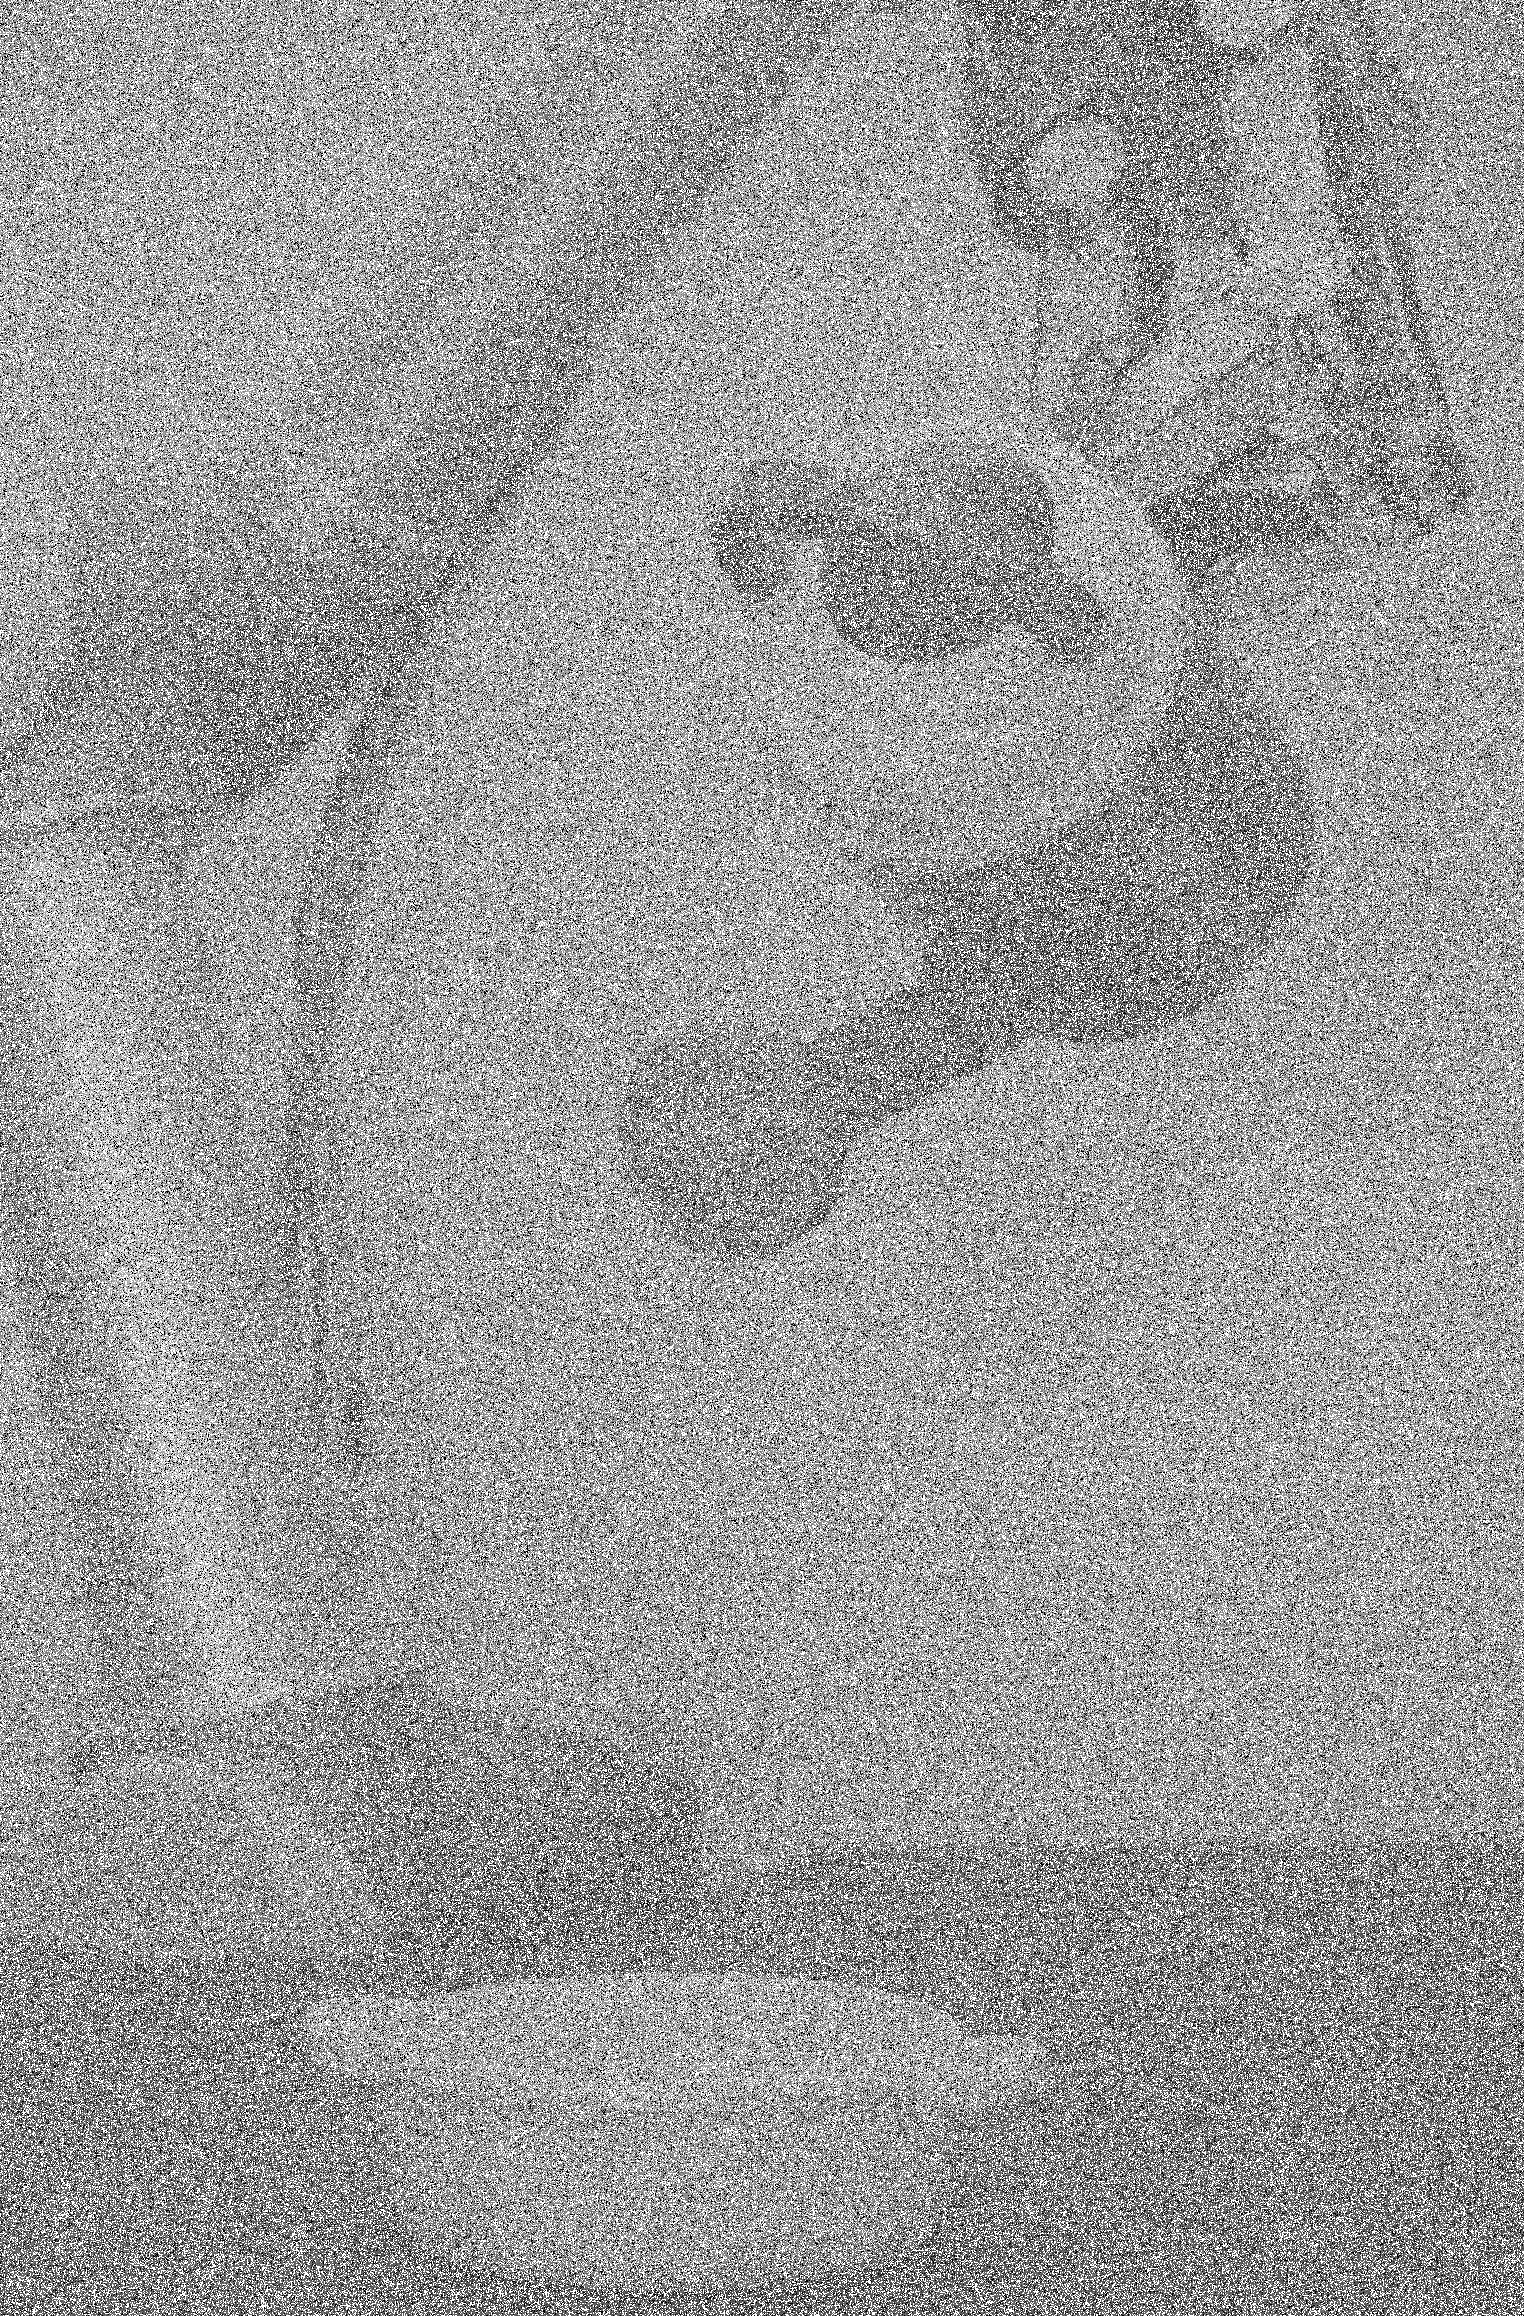
\includegraphics[width=\textwidth]{img2/src.png}
        \caption{The original image}
        \label{fig:img2_src}
    \end{subfigure}
    \begin{subfigure}[b]{0.16\textwidth}
        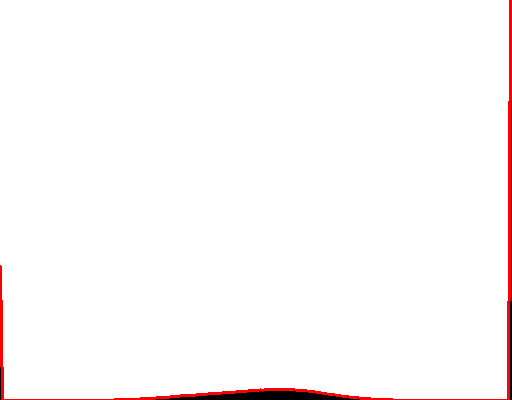
\includegraphics[width=\textwidth]{img2/hist.png}
        \caption{Histogram of the original image}
        \label{fig:img2_hist}
    \end{subfigure}	
\begin{subfigure}[b]{0.16\textwidth}
        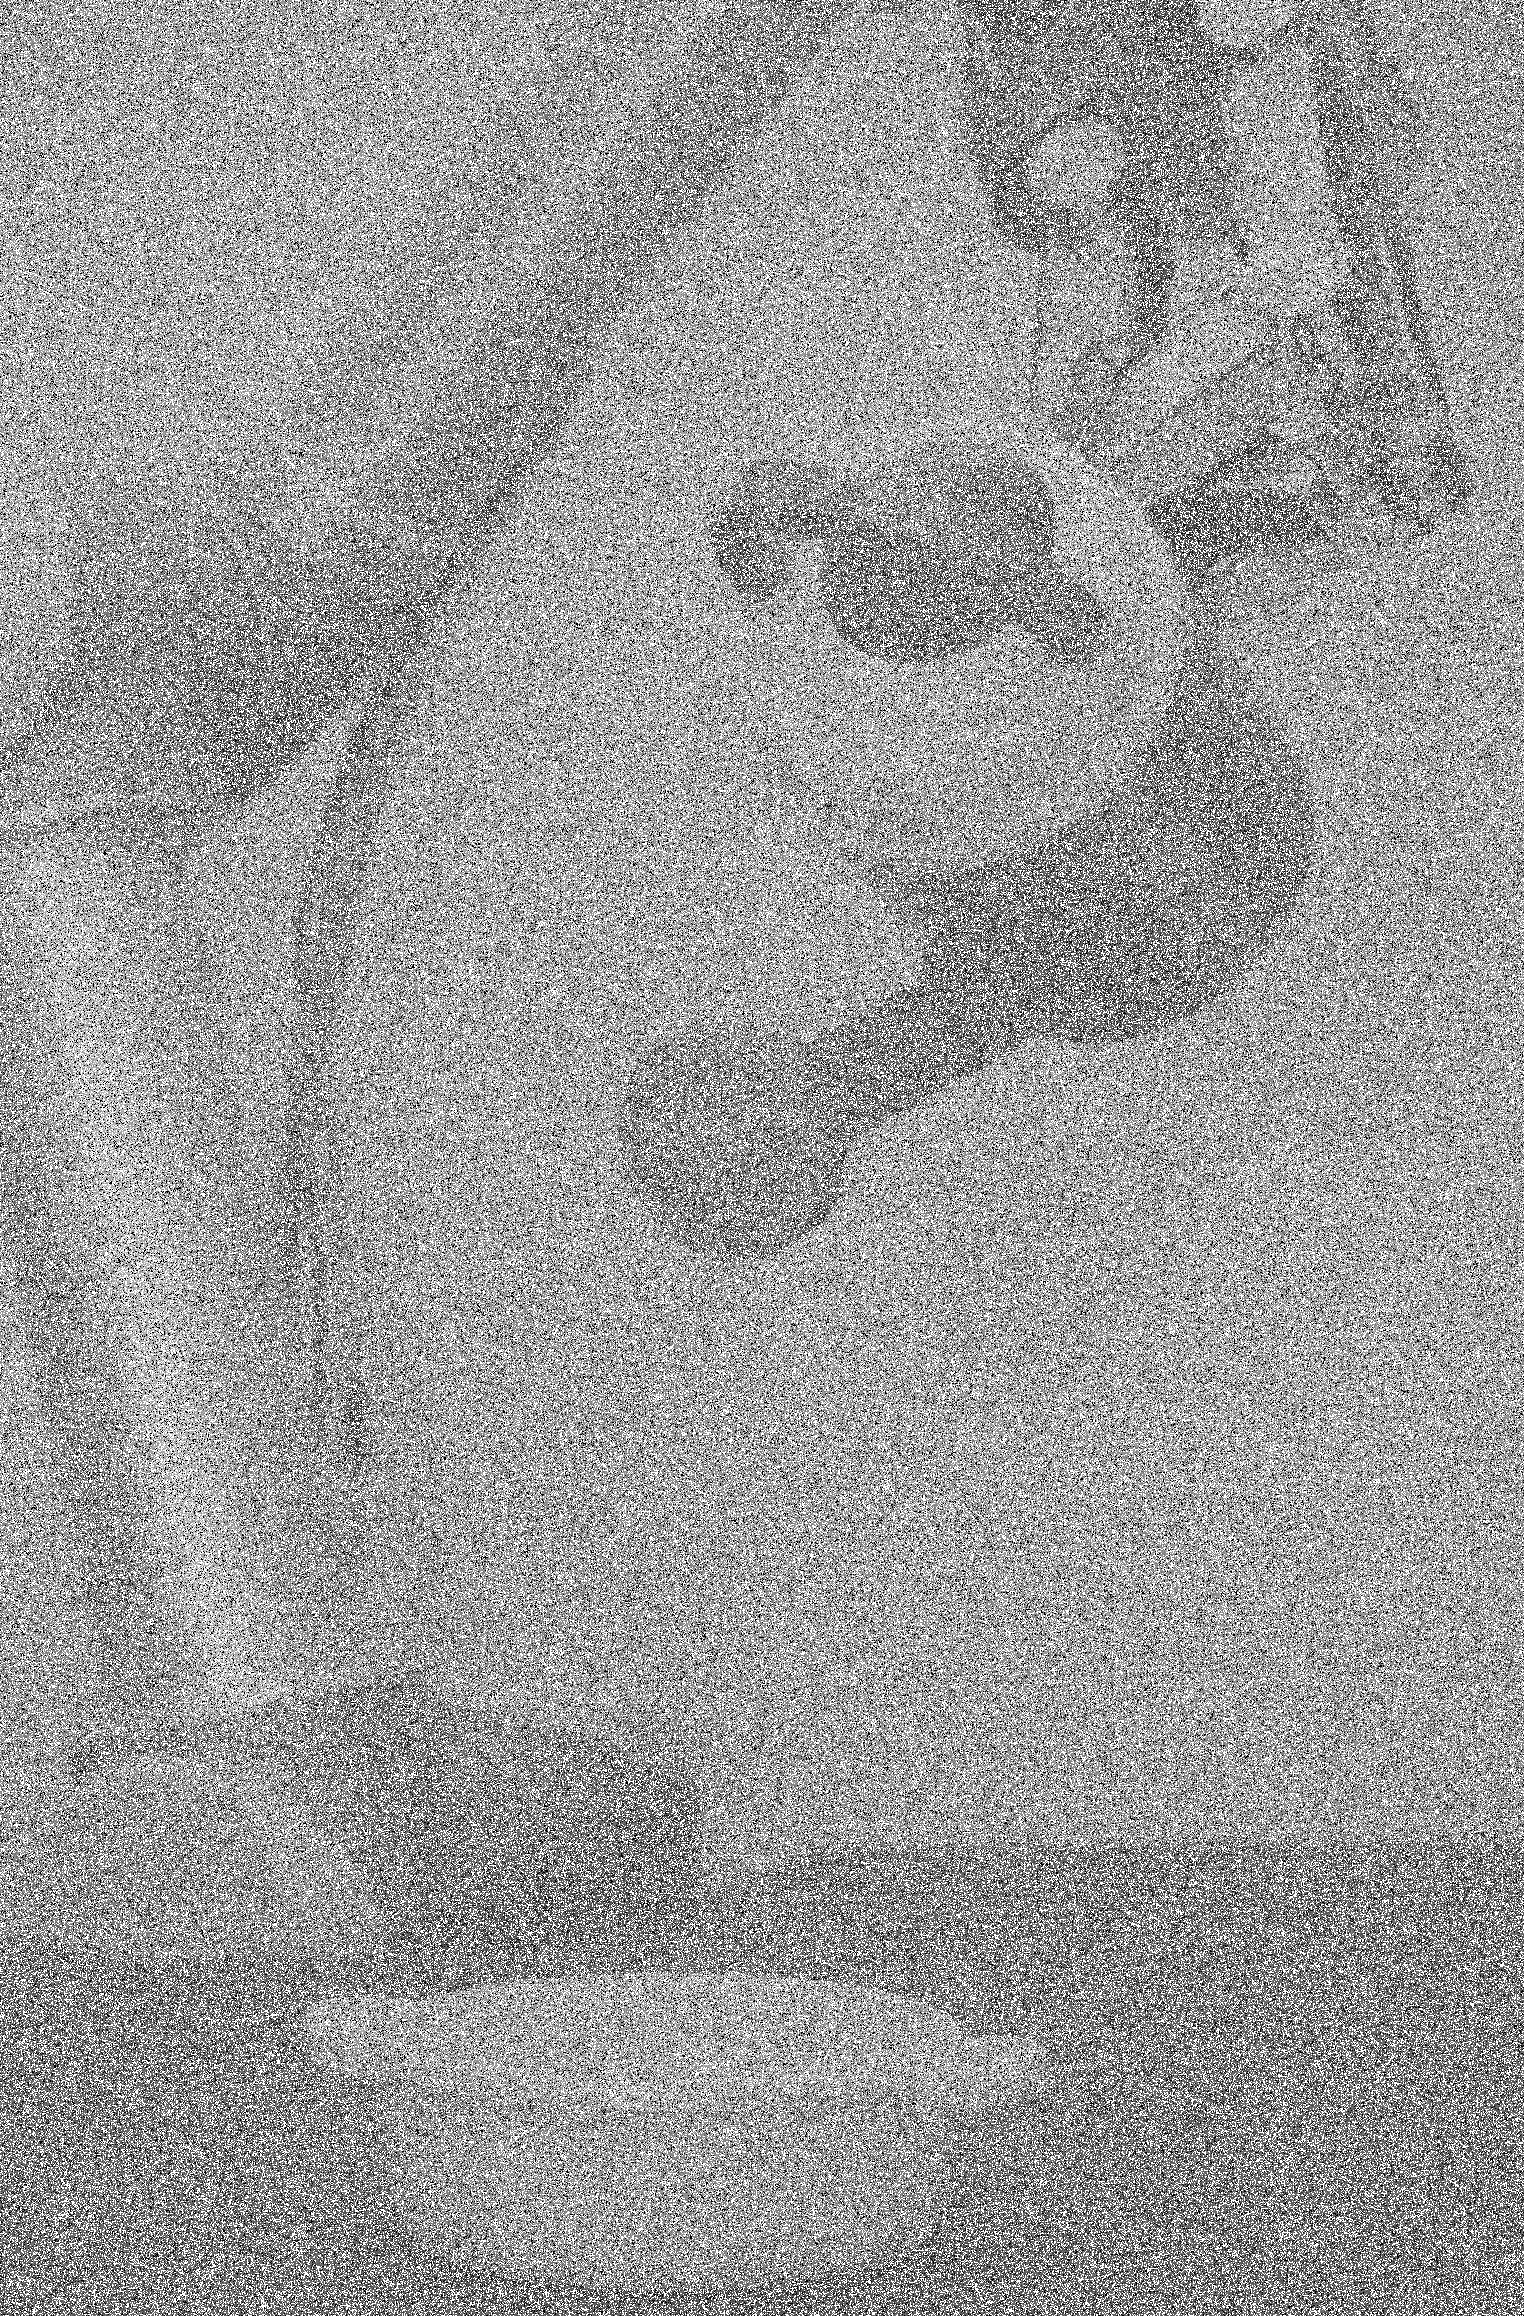
\includegraphics[width=\textwidth]{img2/src.png}
        \caption{The original image}
        \label{fig:img2_src}
    \end{subfigure}
    \begin{subfigure}[b]{0.16\textwidth}
        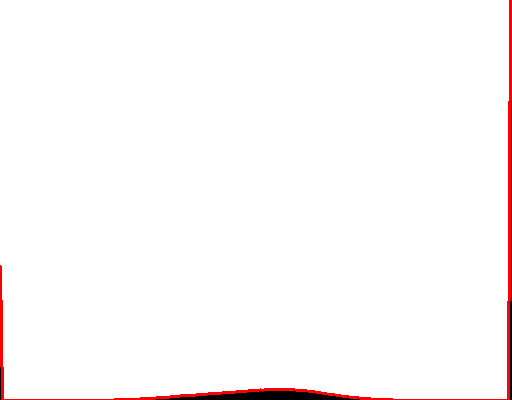
\includegraphics[width=\textwidth]{img2/hist.png}
        \caption{Histogram of the original image}
        \label{fig:img2_hist}
    \end{subfigure}
\end{figure}


From the figure (comming) it can be seen that the filters weakens the effect of the frequency components. Some ringing effect occurs as the image gets filtered with higher order filter. This is due to the transition occuring more abruptly thus resembling the an ideal filter. 

\begin{figure}[H]
	\centering
	\includegraphics[width=0.3\textwidth]{img4/filter_become_ideal2.png}
	\caption{Filter becomes more ideal as the order increases.}
    \label{fig:filter_become_ideal}
\end{figure}


The image which was used for further processing is the output generated by applying a low pass buterworth filter with an $d_0 = 650$ and order of 9. \\
 
 By resembling the output from the filter with original it can be see that the constrast differs a bit compared with the original,  hence contrast streching be applied on to the image, which returns this image. 
 
 \begin{figure}[H]
 \centering
 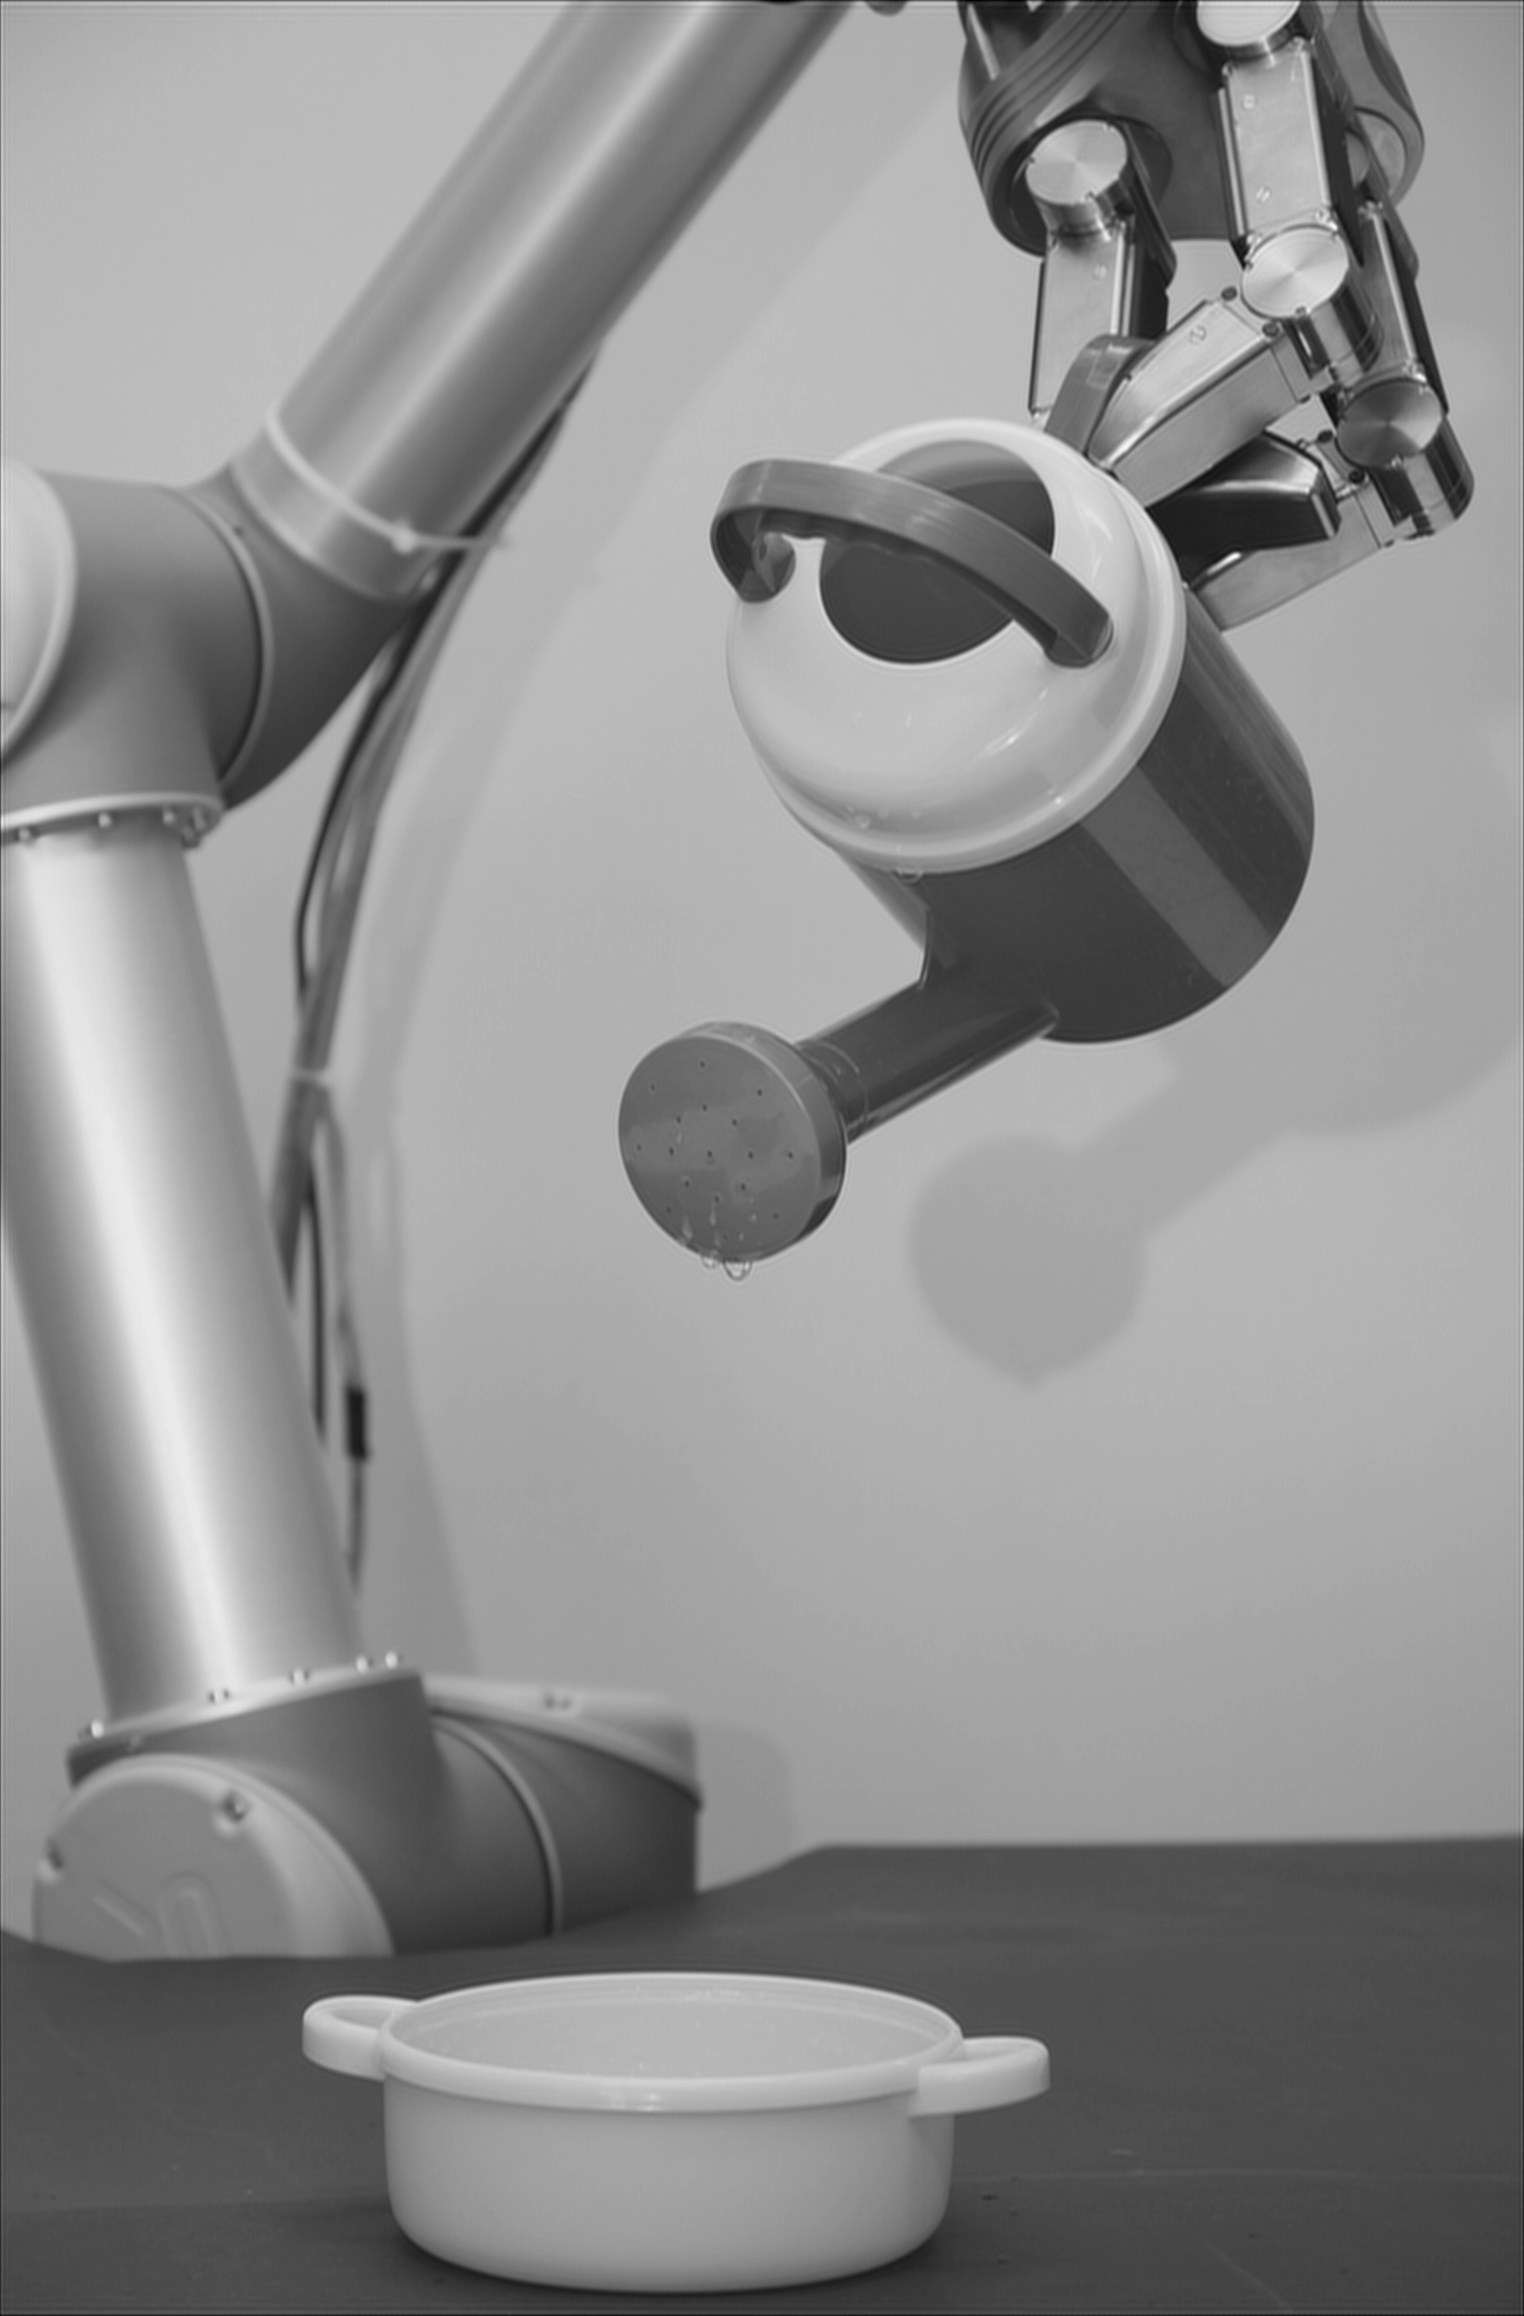
\includegraphics[width=0.3\textwidth]{img4/filteredOutput_6509_contrast_strech.png}
 	\caption{Contrast strecthing applied to the image. }
    \label{fig:filter_become_ideal}
\end{figure} 

At this point it was determined that the image was restored enough, to resemble the original image. 

\begin{figure}[H]
\centering
    \begin{subfigure}[b]{0.24\textwidth}
        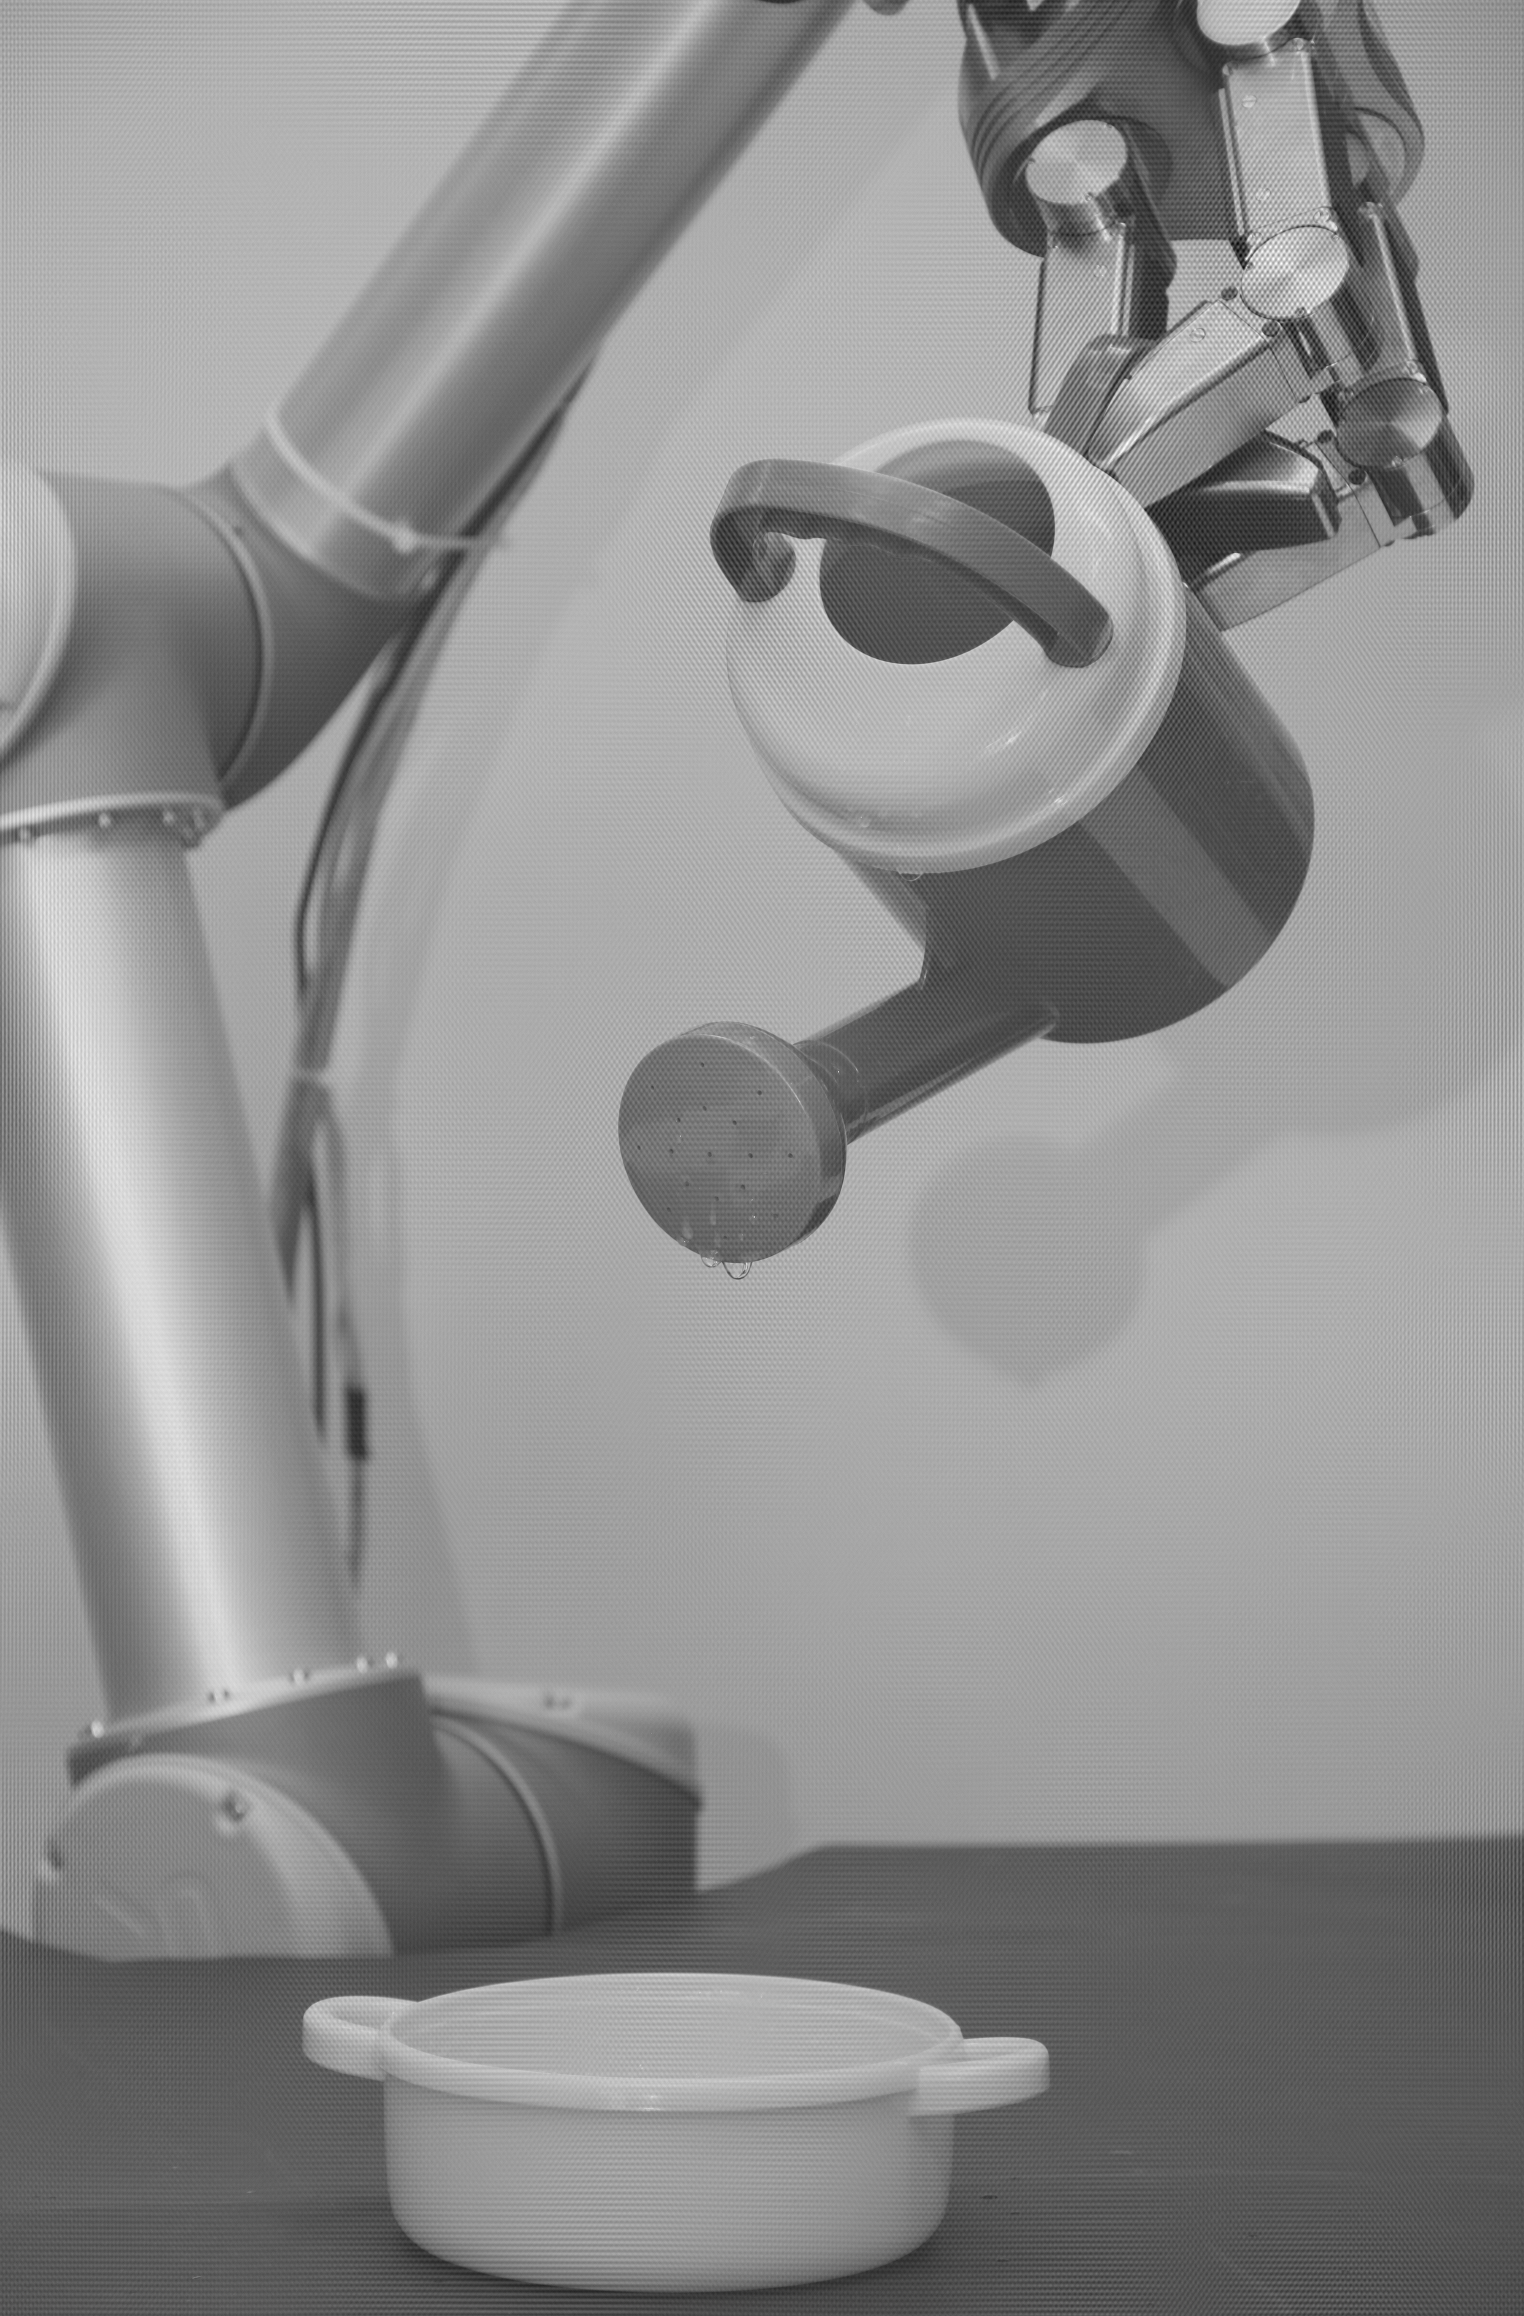
\includegraphics[width=\textwidth]{img4/Image4_2.png}
        \caption{Start image}
        \label{fig:img2_hist}
    \end{subfigure}
	 \begin{subfigure}[b]{0.24\textwidth}
        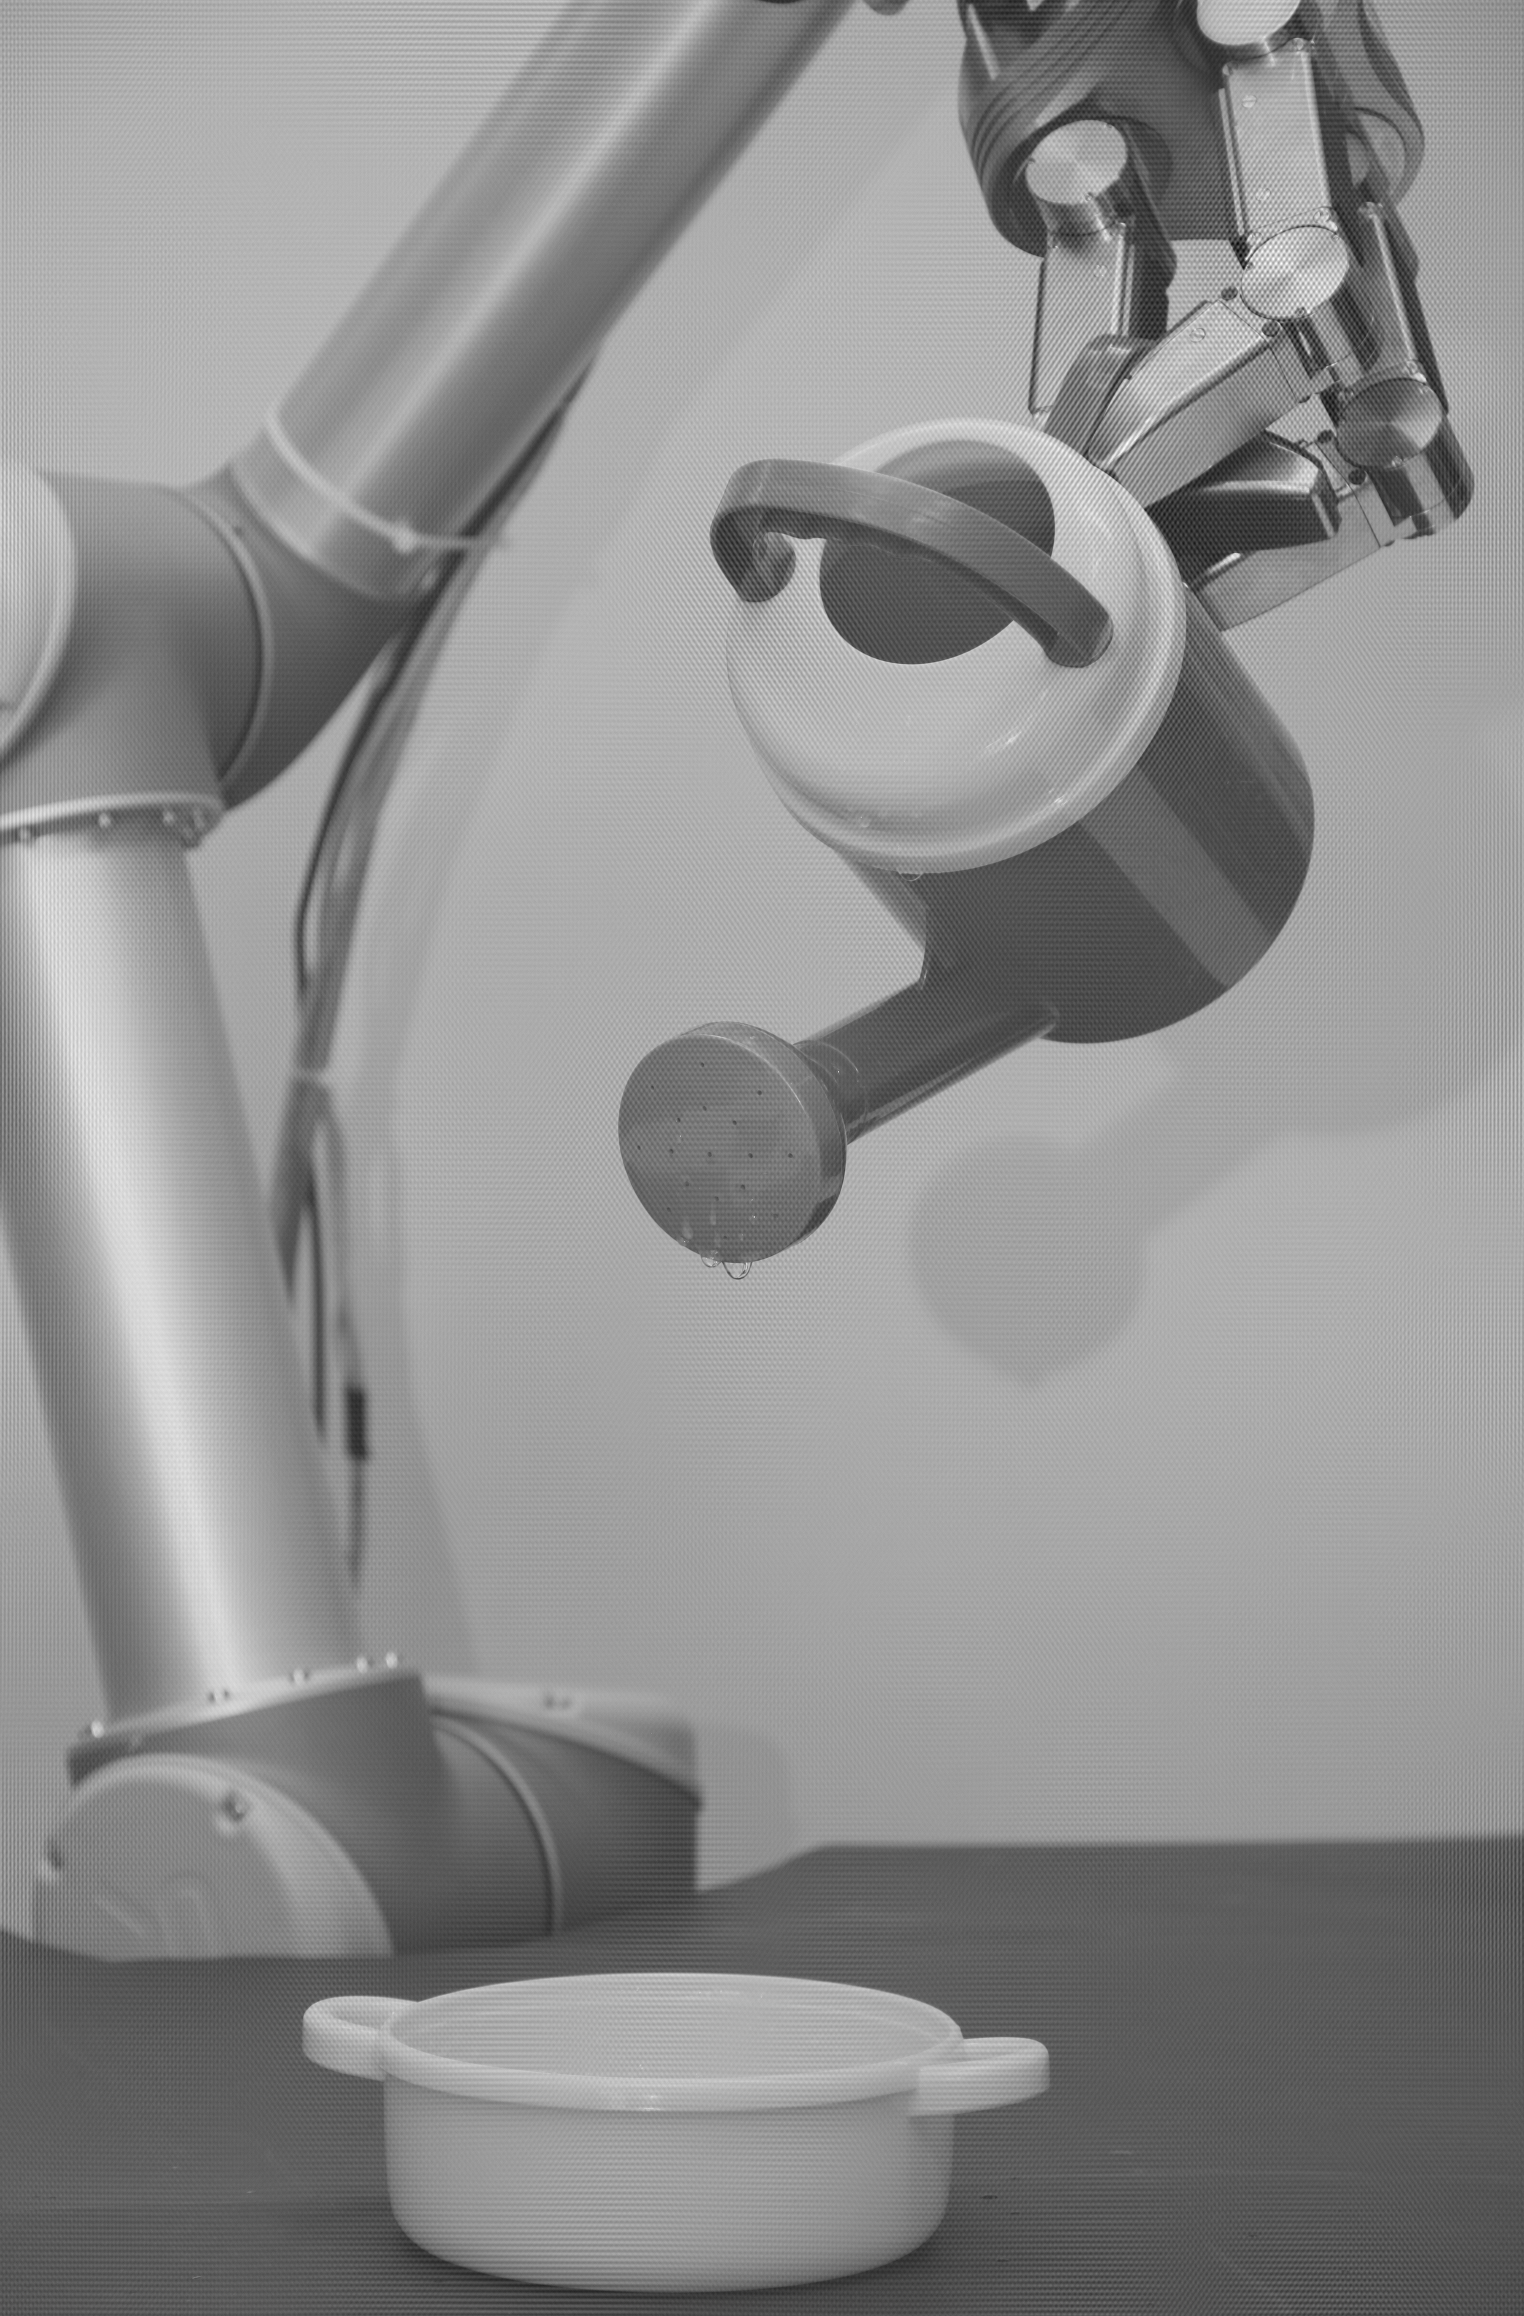
\includegraphics[width=\textwidth]{img4/Image4_2.png}
        \caption{Lowpass filtered}
        \label{fig:img2_src}
    \end{subfigure}
    \begin{subfigure}[b]{0.24\textwidth}
        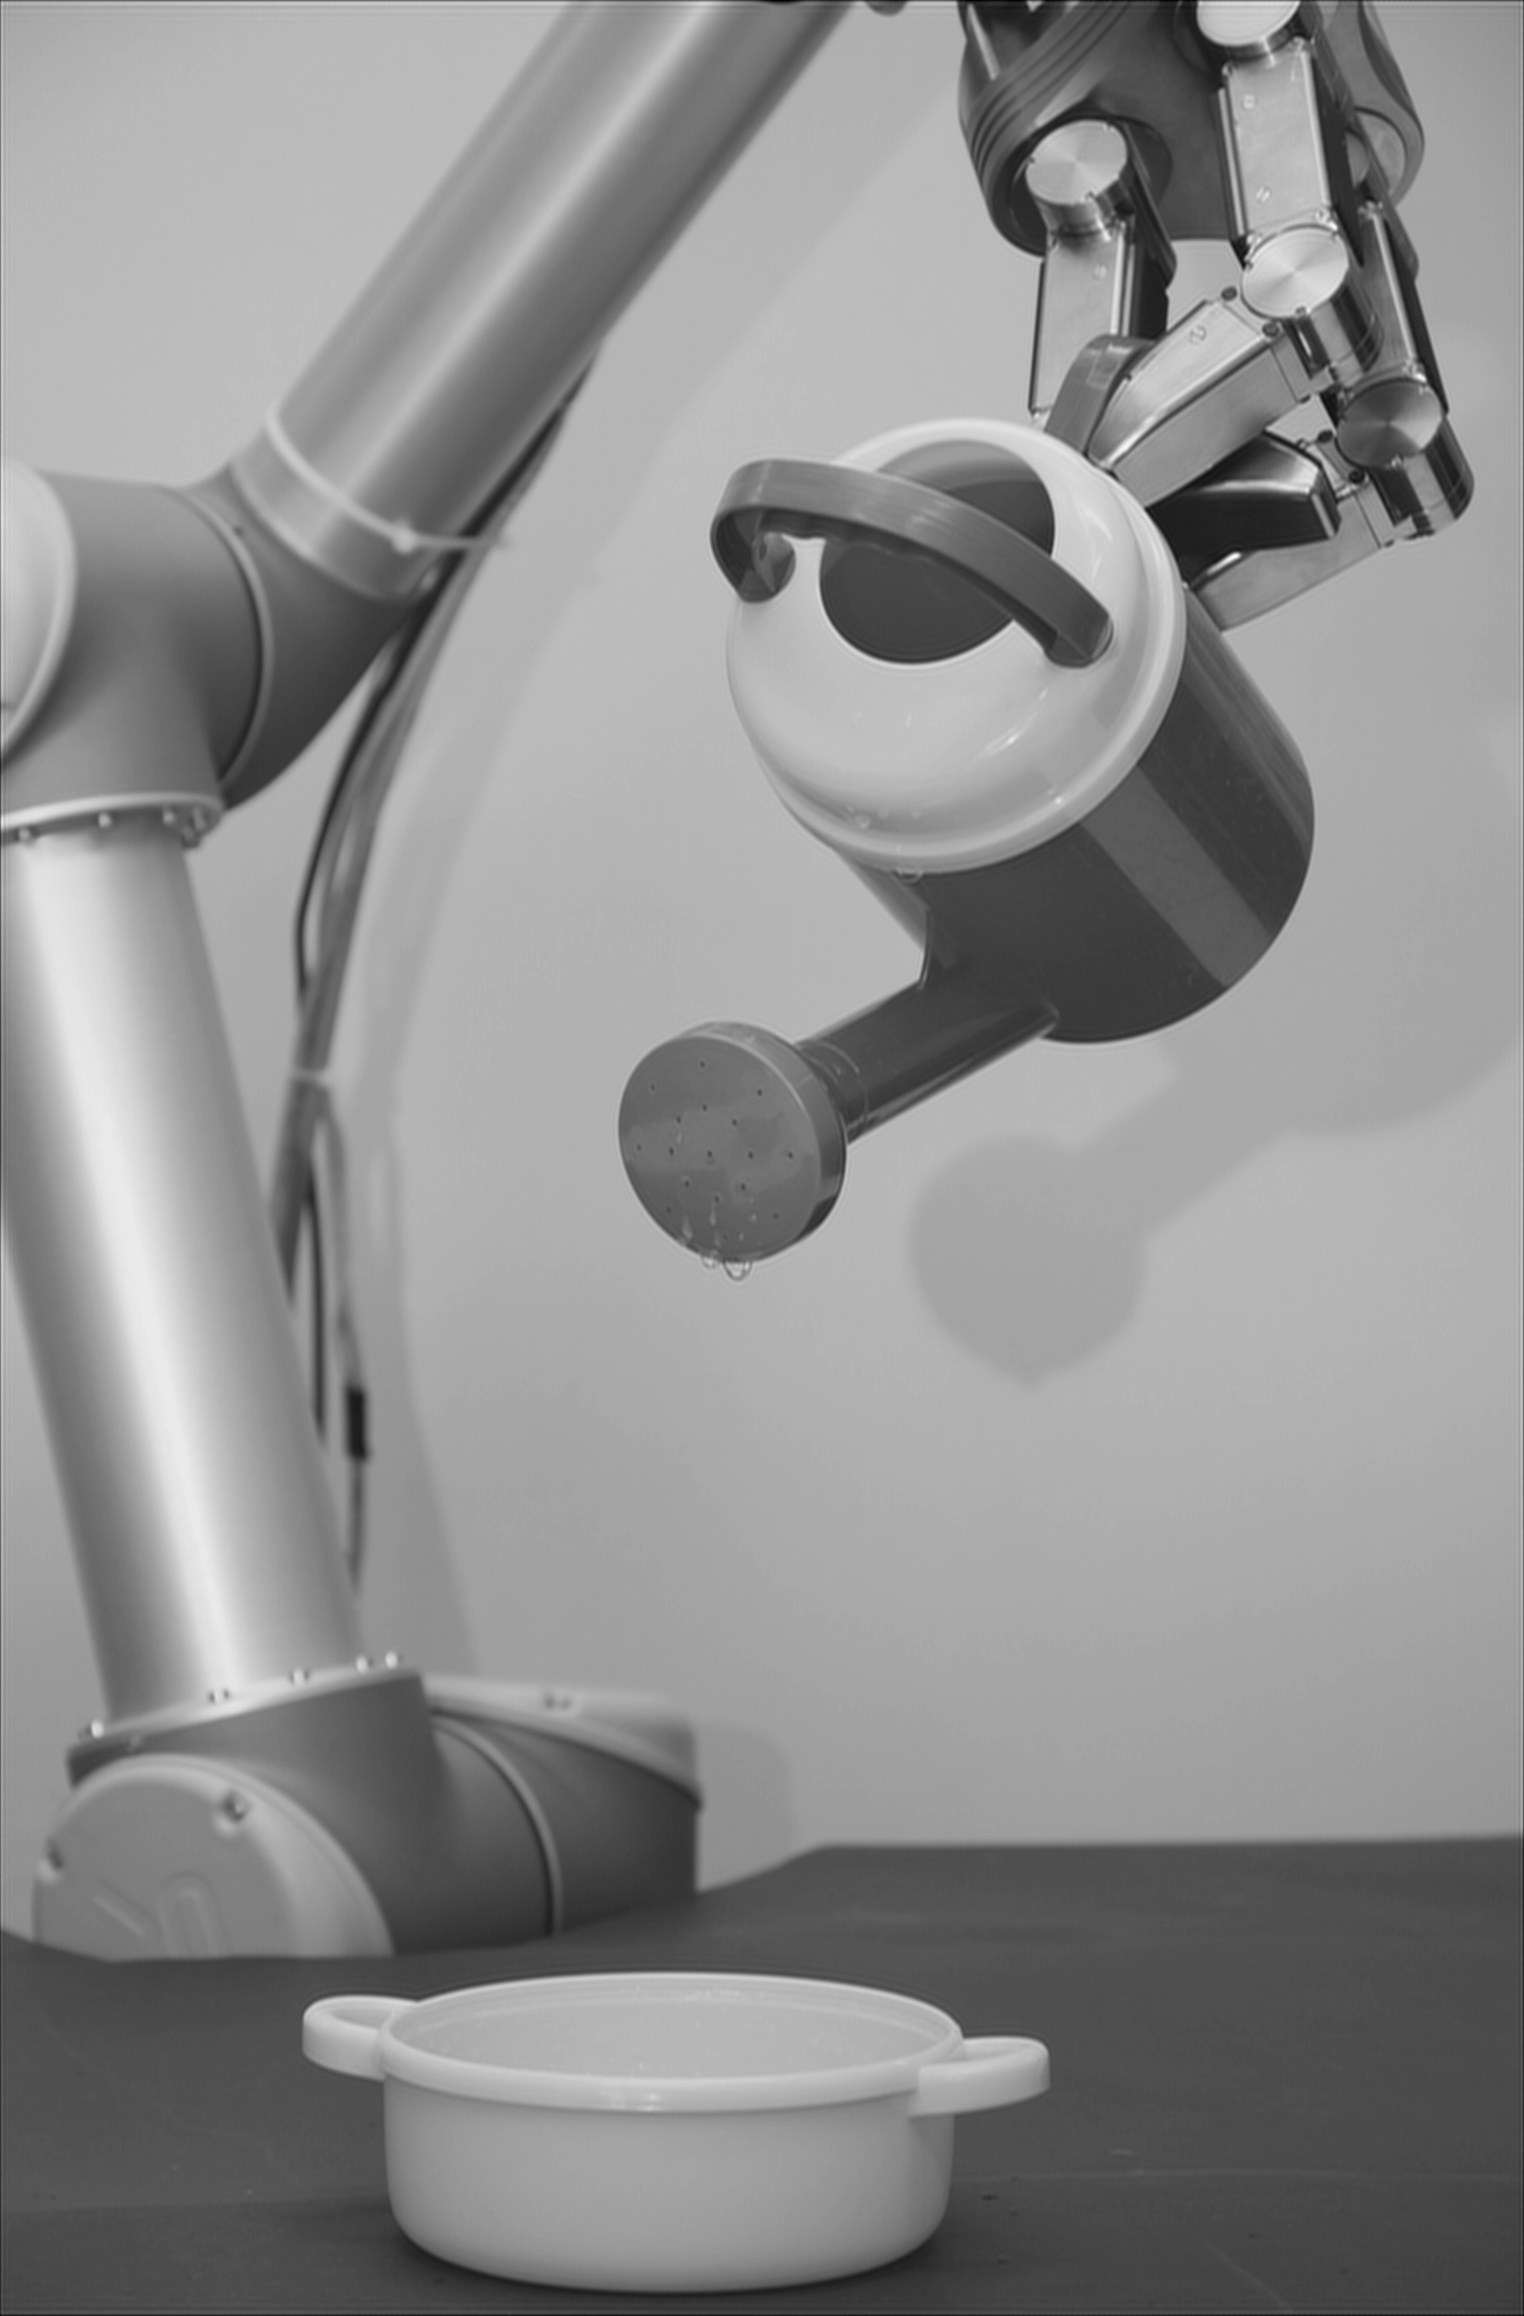
\includegraphics[width=\textwidth]{img4/filteredOutput_6509_contrast_strech.png}
        \caption{Contrast stretched}
        \label{fig:img2_hist}
    \end{subfigure}	
\begin{subfigure}[b]{0.24\textwidth}
        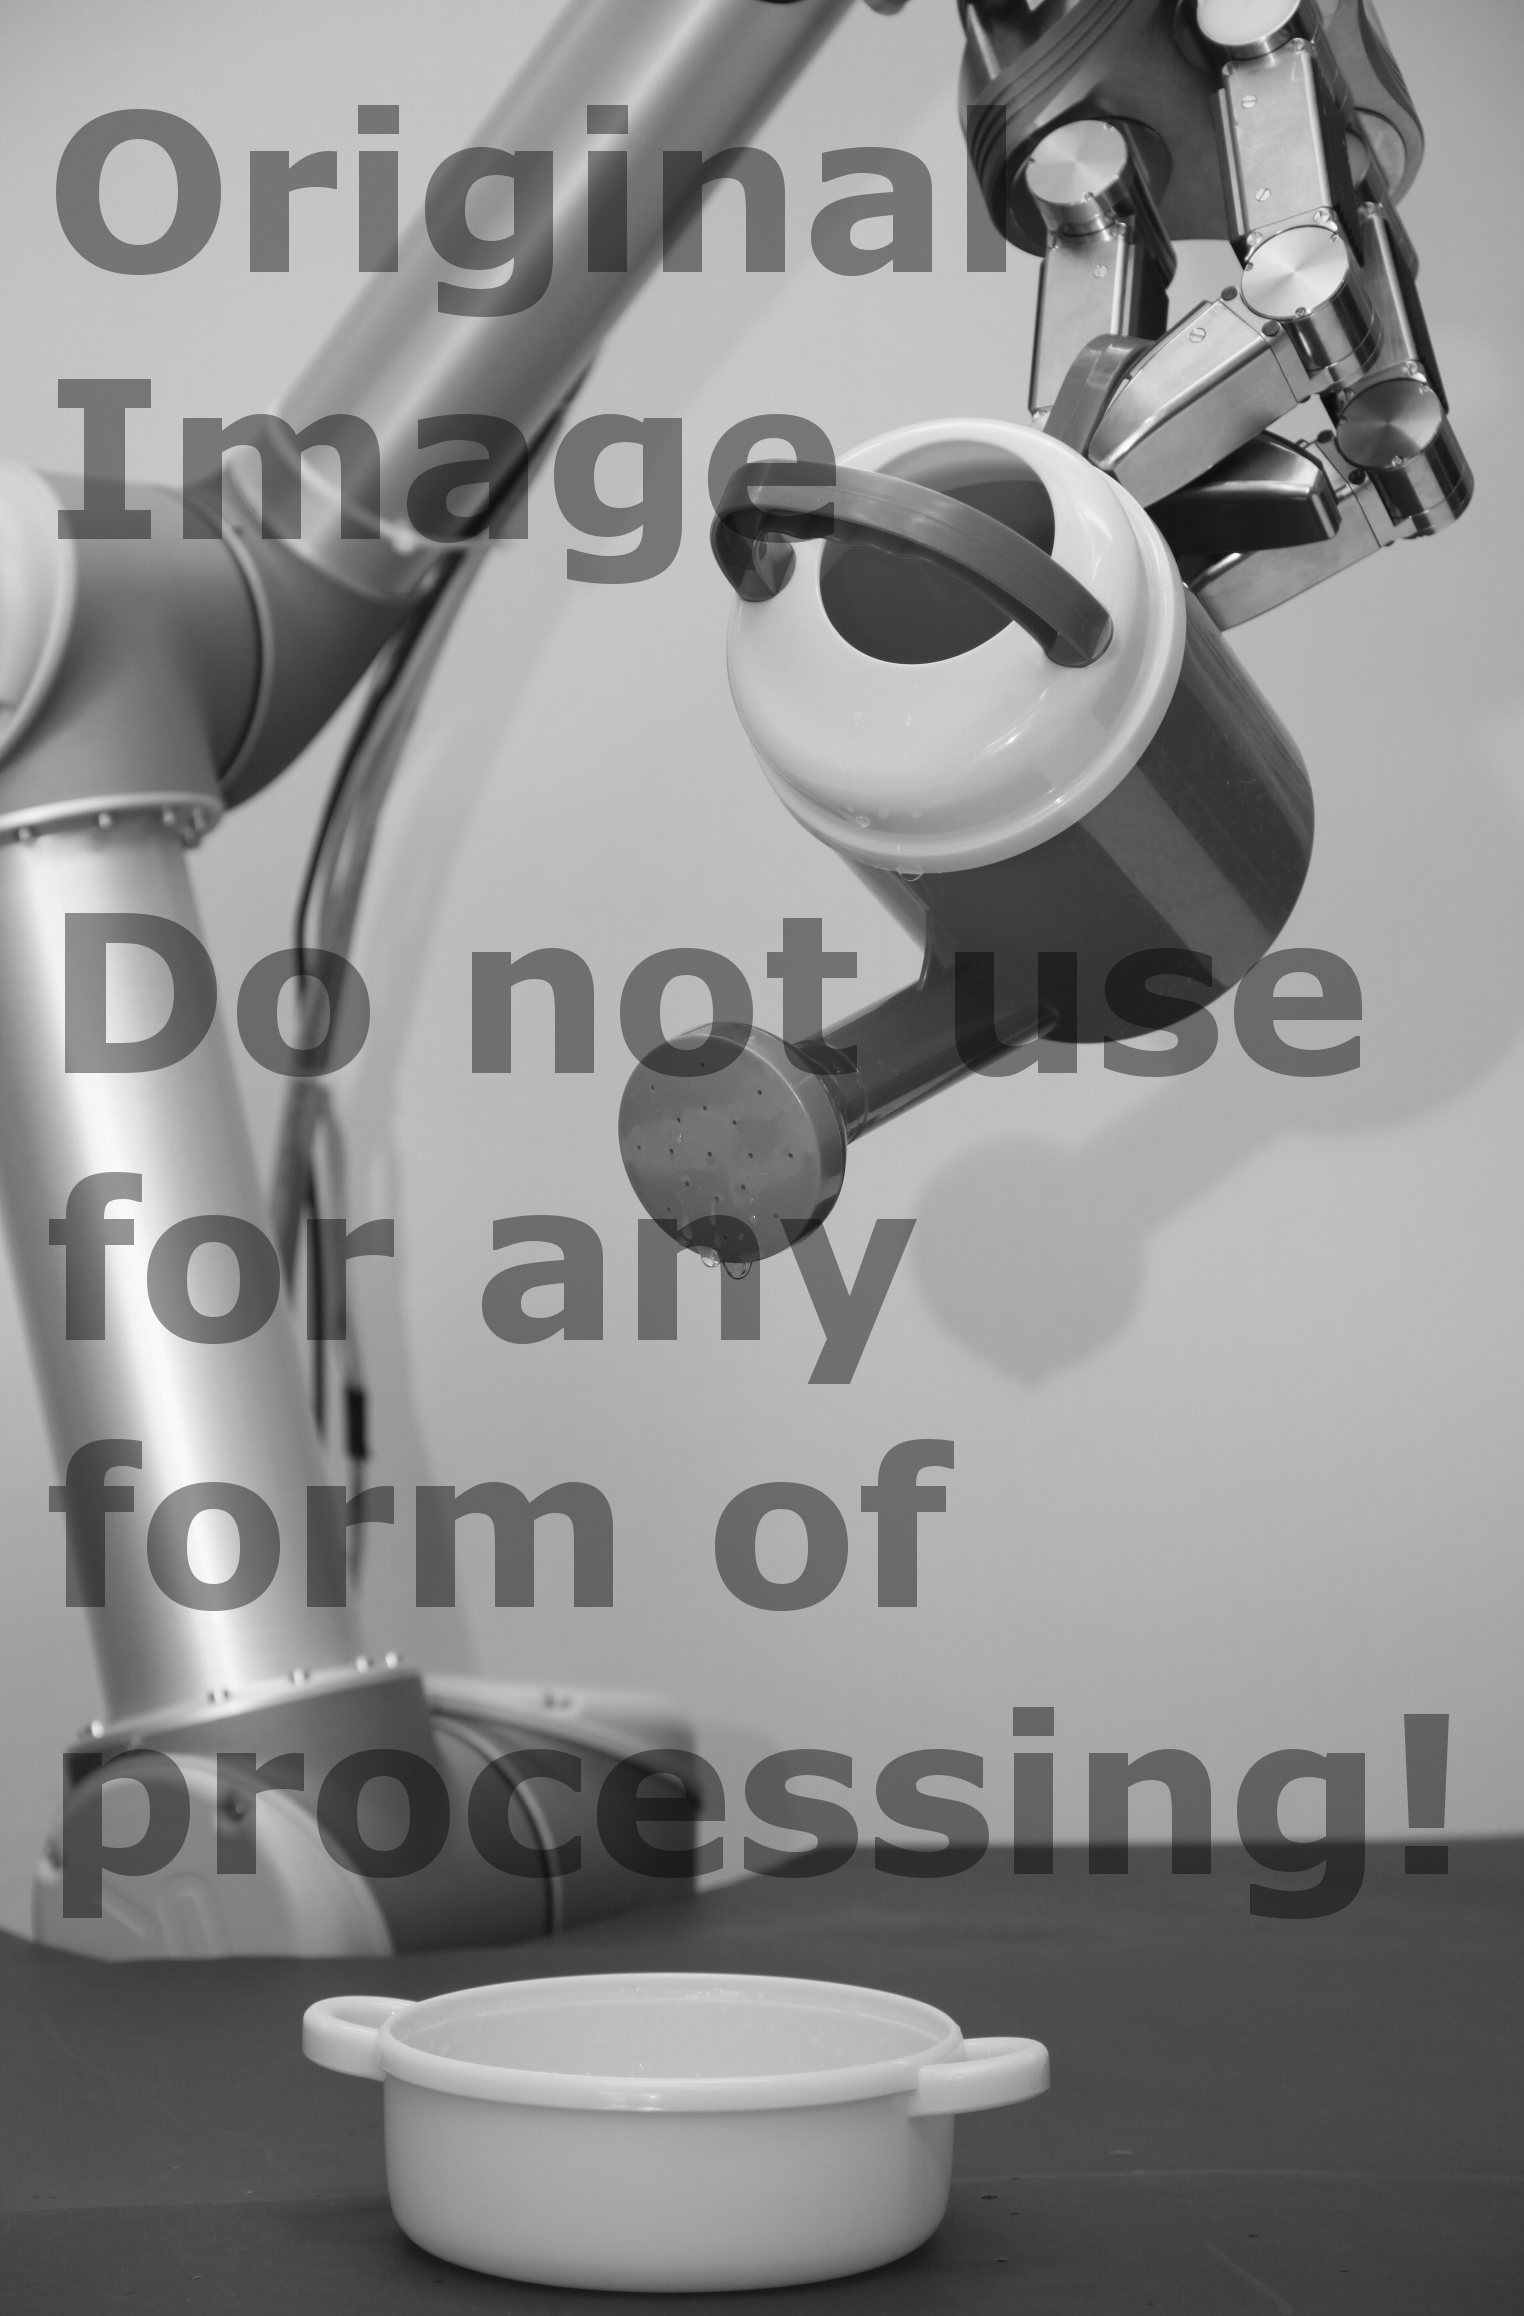
\includegraphics[width=\textwidth]{org.png}
        \caption{The original image}
        \label{fig:img2_src}
    \end{subfigure}
\end{figure}



